%%%%%%%%%%%%%%%%%%%%%%%%%%%%%%%%%%%%%%%%%%%%%%%%%%%%%%%%%%%%%%%%%%%%%%%%%%%%%%%
% Machine Learning IrOx OER Paper %%%%%%%%%%%%%%%%%%%%%%%%%%%%%%%%%%%%%%%%%%%%%
% %%%%%%%%%%%%%%%%%%%%%%%%%%%%%%%%%%%%%%%%%%%%%%%%%%%%%%%%%%%%%%%%%%%%%%%%%%%%%
%
%%%%%%%%%%%%%%%%%%%%%%%%%%%%%%%%%%%%%%%%%%%%%%%%%%%%%%%%%%%%%%%%%%%%%%%%%%%%%%%

% | - __latex_setup__

\documentclass[%
  journal=jacsat,
  manuscript=article,
  % layout=twocolumn,  % Two-column formatting, more compact
  ]{achemso}

% %%%%%%%%%%%%%%%%%%%%%%%%%%%%%%%%%%%%%%%%%%%%%%%%%%%%%%%%%%%%%%%%%%%%%%%%%%%%%
% %%%%%%%%%%%%%%%%%%%%%%%%%%%%%%%%%%%%%%%%%%%%%%%%%%%%%%%%%%%%%%%%%%%%%%%%%%%%%

\usepackage[version=3]{mhchem}  % Formula subscripts using \ce{}
\usepackage{xspace}  % To add space after macros

\usepackage{subcaption}  % Used to create tables
\captionsetup{justification=raggedright,singlelinecheck=false}  % Trying to get the tables a bit more centered

%| - Unused packages, maybe will be necessary later
% \usepackage[table,xcdraw]{xcolor}
% \usepackage[normalem]{ulem}  % Used for underlining and crossing out text
% \usepackage{subfig}  % Support for subfiguress
% \usepackage{multirow}  % Used for tables I think
% \usepackage{hhline}  % Used for making lines in tables I think

% Boolean options
% \usepackage{endfloat}  % 190731 | RF | Put's all figures at the end
% \usepackage{hyperref}  % TEST | Used to reference sections w/ hyperlinks
% __|

% %%%%%%%%%%%%%%%%%%%%%%%%%%%%%%%%%%%%%%%%%%%%%%%%%%%%%%%%%%%%%%%%%%%%%%%%%%%%%
% %%%%%%%%%%%%%%%%%%%%%%%%%%%%%%%%%%%%%%%%%%%%%%%%%%%%%%%%%%%%%%%%%%%%%%%%%%%%%
% - Author List
%%%%%%%%%%%%%%%%%%%%%%%%%%%%%%%%%%%%%%%%%%%%%%%%%%%%%%%%%%%%%%%%%%%%%%%%%%%%%%%
%%
%%
%%
%%%%%%%%%%%%%%%%%%%%%%%%%%%%%%%%%%%%%%%%%%%%%%%%%%%%%%%%%%%%%%%%%%%%%%%%%%%%%%%


% | - @Raul Flores
\author{Raul A. Flores}
\affiliation[SUNCAT]{
  SUNCAT Center for Interface Science and Catalysis,
  Department of Chemical Engineering,
  Stanford University,
  Stanford 94305,
  California,
  USA
  }
\email{flores12@stanford.edu}
% __|

% | - @Christopher Paolucci
\author{Christopher Paolucci}
\affiliation[UVA]
{
  Department of Chemical Engineering,
  University of Virginia,
  Charlottesville,
  Virginia 22903,
  United States
  }
\email{cp9wx@virginia.edu}
% __|

% | - Ankit Jain
\author{Ankit Jain}
\affiliation[DTU]
{
  Department of Physics,
  Technical University of Denmark,
  Lyngby,
  Denmark
  }
\email{temp_temp_ankits_email_address_temp_temp@dtu.dk}
% __|

% | - Ziyun Wang
% \author{Zhyun}
% \affiliation[SUNCAT]
% {
% SUNCAT Center for Interface Science and Catalysis,
% Department of Chemical Engineering,
% Stanford University,
% Stanford,
% California,
% United States
% }
% \email{temp_temp_ankits_email_address_temp_temp@dtu.dk}s
% __|


\author{Kirsten T. Winther}
\affiliation[SUNCAT]{
  SUNCAT Center for Interface Science and Catalysis,
  Department of Chemical Engineering,
  Stanford University,
  Stanford 94305,
  California,
  USA
  }



% | - Muratahan Aykol
\author{Muratahan Aykol}
\affiliation[TRI]
{
  Toyota Research Institute,
  Los Altos,
  CA 94022,
  USA
  }
\email{muratahan.aykol@tri.global}
% __|

% | - Jens Norskov
\author{Jens K. N{\o}rskov}
\affiliation[DTU]
{
  Department of Physics,
  Technical University of Denmark,
  Lyngby,
  Denmark
  }
\email{jkno@dtu.dk}
% __|

% | - @Michal Bajdich
\author{Michal Bajdich}
\affiliation[SLAC]{
  SUNCAT Center for Interface Science and Catalysis,
  SLAC National Accelerator Laboratory,
  Menlo Park,
  CA 94025,
  USA
  }
\email{bajdich@slac.stanford.edu}
% __|

% | - Thomas Bligaard
\author{Thomas Bligaard}
\affiliation[SLAC]{
  SUNCAT Center for Interface Science and Catalysis,
  SLAC National Accelerator Laboratory,
  Menlo Park,
  CA 94025,
  USA
  }
\email{bligaard@stanford.edu}
% __|


% - Custom Macros
%%%%%%%%%%%%%%%%%%%%%%%%%%%%%%%%%%%%%%%%%%%%%%%%%%%%%%%%%%%%%%%%%%%%%%%%%%%%%%%
% Latex Macros
%%%%%%%%%%%%%%%%%%%%%%%%%%%%%%%%%%%%%%%%%%%%%%%%%%%%%%%%%%%%%%%%%%%%%%%%%%%%%%%

% Chris commenting command
\newcommand{\chris}[1]{\textcolor{red}{#1}}
\newcommand{\comment}[1]{\textcolor{red}{\textbf{#1}}}


% #########################################################
% Chemical formulas #######################################
% IrOx, IrO3, IrO2
\def \IrOx {IrO\textsubscript{x}\xspace}
\def \IrOthree {IrO\textsubscript{3}\xspace}
\def \IrOtwo {IrO\textsubscript{2}\xspace}

% RhO2
\def \RhOtwo {RhO\textsubscript{2}\xspace}

% rutile-IrO2, alpha-IrO3, rutile-IrO3, beta-IrO3
\def \rIrOtwo {R-\ce{IrO_2}\xspace}
\def \aIrOthree {$\alpha$-\ce{IrO_3}\xspace}
\def \rIrOthree {R-\ce{IrO_3}\xspace}
\def \bIrOthree {$\beta$-\ce{IrO_3}\xspace}

% Aqueous IrO4- phase
\def \IrOfourm {\ce{IrO_{4}^{-}}\xspace}

% AB2 and AB3 (ABO3 too)
\def \ABtwo {AB\textsubscript{2}\xspace}
\def \ABthree {AB\textsubscript{3}\xspace}
\def \ABOthree {AB\textsubscript{3}\xspace}

% #########################################################
% Adsorption energies #####################################

% ΔE_OH, ΔE_O, ΔE_OOH
\def \DEOH {$\Delta$E\textsubscript{OH}\xspace}
\def \DEO {$\Delta$E\textsubscript{O}\xspace}
\def \DEOOH {$\Delta$E\textsubscript{OOH}\xspace}

% ΔG_OH, ΔG_O, ΔG_OOH
\def \DGOH {$\Delta$G\textsubscript{OH}\xspace}
\def \DGO {$\Delta$G\textsubscript{O}\xspace}
\def \DGOOH {$\Delta$G\textsubscript{OOH}\xspace}

% ΔG_O-ΔG_OH
\def \DGOmOH {$\Delta$G\textsubscript{O}-$\Delta$G\textsubscript{OH}}


% #########################################################
% Enthalpy of formation ΔH_f ##############################
\def \DHf {$\Delta$H\textsubscript{f}\xspace}
\def \DGf {$\Delta$G\textsubscript{f}\xspace}

% #########################################################
% V vs RHE notation #######################################
\def \VRHE {$V\textsubscript{RHE}$\xspace}

% Angstrom
\newcommand{\angstrom}{\textup{\AA}}

% Tilde ~
\newcommand{\mytilde}{\raise.17ex\hbox{$\scriptstyle\mathtt{\sim}$}}

% __|

% Article Title ***************************************************************
\title[ML discovered \IrOx phases]{
  Active Learning Discovery of Oxidized and Active \IrOx Phases}

\begin{document}

% | - TOC Figure
\begin{tocentry}
\begin{center}
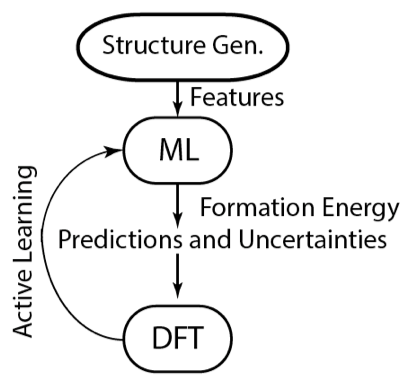
\includegraphics[height=3.5cm]{02_figures/al_diagram/Surrogate_model}
\end{center}
\end{tocentry}
% __|


% #############################################################################
% | - MAIN DOCUMENT ***********************************************************
% - 00 | Abstract *************************************************************
\begin{abstract}
%%%%%%%%%%%%%%%%%%%%%%%%%%%%%%%%%%%%%%%%%%%%%%%%%%%%%%%%%%%
% Abstract %%%%%%%%%%%%%%%%%%%%%%%%%%%%%%%%%%%%%%%%%%%%%%%%
% %%%%%%%%%%%%%%%%%%%%%%%%%%%%%%%%%%%%%%%%%%%%%%%%%%%%%%%%%
%
%%%%%%%%%%%%%%%%%%%%%%%%%%%%%%%%%%%%%%%%%%%%%%%%%%%%%%%%%%%

%| - MY OLD VERSION
% %
% Machine learning (ML) based surrogate models have become an increasingly common tool in the field computational materials discovery to overcome the relative expense of \latin{ab-initio} density functional theory (DFT).
% %
% Training such models on expansive DFT data sets has been used to discover new materials in the vast space of material compositions.
% %
% % COMBAK This is probably too strong
% However, surrogate model applications to the structural space of bulk crystals, \latin{i.e.} polymorphs, remain relatively unexplored.
% %
% Herein, we report on an active learning (AL) framework that searches for the most stable polymorph of a chemical space by utilizing a surrogate model which is sequentially updated on the fly with generated DFT data.
% %
% The model searches within a candidate data set of crystal motifs sourced from publicly available materials databases.
% %
% We demonstrate the efficacy of this AL-accelerated methodology by discovering the most stable polymorphs of \IrOtwo and \IrOthree within the candidate space with DFT calculations of only a fraction of the candidate space.
% % 7 out of the 10 most stable crystal structures for \IrOtwo and \IrOthree with less than 50 DFT calculations.
% %
% % COMBAK TODO Update number of unique polymorphs discovered to something more meaningful
% % Let's report how many meta-stable IrO2/3 we discovered, much better than how it is currently phrased
% For \IrOtwo, we reaffirm the rutile phase as the globally stable polymorph, while also finding \mytilde200 polymorphs that are within the synthesizability limit.
% %
% For \IrOthree we discovered ~70 unique metastable polymorphs, with \mytilde20 that are more stable than anything previously reported.
% %
% The globally stable polymorph of \IrOthree is a FeF\textsubscript{3} structure type polymorph with a space group number of 167.
% %
% % There are 10 IrO3 polymorphs within 0.2 eV/atom of the lowest structure and 5 IrO3 polymorphs within 0.1 eV/atom of the lowest structure
% % Of these 10, how many were unknown? Maybe 8ish? TODO double check
% %
% %For \IrOthree, we discover 10 previously unknown polymorphs, and the most stable
% %$\alpha$-AlF\textsubscript{3} type and a rutile-like \IrOthree structure with stabilities lower than 0.2 per atom than anything known to date.
% %
% Based on the above results, we constructed a revised bulk Pourbaix diagram of the Ir-H\textsubscript{2}O system by including \IrOthree, and show that our \aIrOthree phase is the dominant and fully stable phase under acidic oxygen evolution reaction (OER) conditions.
% %
% % COMBAK "the OER" or just "OER"
% Using a thermodynamic criteria for the activity towards the OER we find that the above stable \IrOthree polymorphs have significantly lower theoretical overpotentials than the rutile \IrOtwo phase.
% %
% This elevated catalytic activity is due to the weaker and more ideal binding of the OER intermediates on the more oxidized \IrOthree surfaces.
% %
% % TODO Less cheesy closing thoughts
% This work opens up the possibility of drastically accelerating the discovery of novel crystal structure motifs and has implications towards high through-put catalyst discovery efforts.

%__|





%
Materials science primarily studies the relationship between the structure and functionality of materials,
where the knowledge of viable polymorphic forms of crystals at a given chemical composition plays an indispensable role.
%
Machine-learning based surrogate models have the potential to accelerate this process of creating the knowledge-base for materials polymorphs for target applications in under-explored chemistries.
%
Herein, we report on a sequential, active-learning (AL) accelerated ab-initio study for the identification of novel and stable \IrOx (x=2 or 3) polymorphs,
and the subsequent thermochemical analyses of the activity of these discovered structures towards the oxygen evolution reaction (OER).
%
We demonstrate that compared to a random search,
the AL framework at more than doubles the efficiency of using DFT to find stable polymorphs out of a large array of prototypical structures.
%
We find nearly \num{200} and \num{70} unique polymorphs within the thermodynamic synthesizability limits of \IrOtwo and \IrOthree, respectively,
while validating the rutile ground state for the former and finding a new \ce{FeF_{3}}-like ground state for the latter (\aIrOthree).
%
An analysis of the structural properties of these metastable polymorphs reveals that octahedral local coordination environments are preferred for all low energy structures.
%
Subsequent Pourbaix and thermochemical analyses with this \aIrOthree phase show that it is fully stable under acidic OER conditions,
and delivers lower theoretical overpotentials compared to \rIrOtwo due to weaker and more ideal binding of the OER intermediates on its oxidized surfaces.

\end{abstract}

% - 01 | Introduction *********************************************************
\section{Introduction}
%%%%%%%%%%%%%%%%%%%%%%%%%%%%%%%%%%%%%%%%%%%%%%%%%%%%%%%%%%%%%%%%%%%%%%%%%%%%%%%
% Introduction %%%%%%%%%%%%%%%%%%%%%%%%%%%%%%%%%%%%%%%%%%%%%%%%%%%%%%%%%%%%%%%%
% %%%%%%%%%%%%%%%%%%%%%%%%%%%%%%%%%%%%%%%%%%%%%%%%%%%%%%%%%%%%%%%%%%%%%%%%%%%%%
%
% Key points:
%   * Materials are composed of their "stoichiometry" and their "structure"
%   * 3N dimensional Cartesian space of coordinates is prohibitelvey large
%   * Our candidate space generation leverages symmetry to produce a set of
%     structurally unique and well distributed (across the high dim. 3N space)
%     polymorphs
%   * Mention other methods for bulk crystal structure Discovery
%     - simulated annealing
%     - paper that Hammer put out (R58)
%%%%%%%%%%%%%%%%%%%%%%%%%%%%%%%%%%%%%%%%%%%%%%%%%%%%%%%%%%%%%%%%%%%%%%%%%%%%%%%



% ################################# Paragraph #################################
% %%%%%%%%%%%%%%%%%%%%%%%%%%%%%%%%%%%%%%%%%%%%%%%%%%%%%%%%%%%%%%%%%%%%%%%%%%%%%
% * General intro into problem, give proper context
% * Make the point that structure has been all but ignored in recent years by the big-data/ML material science community (OQMD MP as examples)
%
% OUTLINE:
%  * Solving for crystal structures in a generally difficult problem
%  * It's an important problem to solve because all chemical/physical properties of a material are fundementally linked to the atomic structure.
%  * Although we've seen a lot of work in the past ~10 years from material science groups leveraging recent advances in big-data, ML, cheaper computational resources, high-throughput screening, materials databases, etc.
%    * Most of the focus has been on exploring compositionas and not structure
% %%%%%%%%%%%%%%%%%%%%%%%%%%%%%%%%%%%%%%%%%%%%%%%%%%%%%%%%%%%%%%%%%%%%%%%%%%%%%
% | - Paragraph start
% TODO this intro sentence will be a reference dump for literature in crystal structure prediction
Predicting the thermodynamically favorable crystal structures for an arbitrary inorganic system remains a challenging problem in computational material science.\cite{Woodley2008}
%
% Experimentally synthesized inorganic materials often conform to the global minimum energy structure (or similarly stable meta-stable phases).
%
When simulations are used to guide the search for new materials, the stable and meta-stable crystal structures, \latin{i.e.} polymorphs,  above the convex hull of stability must be known in order to predict the material properties.\cite{}
%
% Structure vs. composition enumeration (composition done to death)
% Give example of how over represented some motifs are
% 188,000 systems with identical prototype ABO2 perovskites structure (~50 %)
% Not sure what to cite for this, example is sufficient
Although there have been numerous examples in recent years of machine learning algorithms applied towards the prediction of formation energies of large \latin{ab-initio} data sets,
these data sets are biased towards common structures and varying composition space.\cite{}
% NUMBER
For example, roughly half of the entries (\mytilde\num{200000}) in The Open Quantum Materials Database (OQMD) correspond to ternary-alloy combinations in the same close-packed cubic structure.\cite{Kirklin2015}
%have identical structures corresponding to ABO3 Perovskites.
% Should we say that enumerating comp. is easy and struct. is hard?
As such, these efforts have been primarily concerned with the enumeration of composition (elemental identity and stoichiometries) and less so with the exploration of structural diversity.
%
% There are way more papers in the general area of GO than these
% I'm leaning away from framing as a "structural-diversity" problem with the databases and more so as a method of global optimization
% In the past, various groups have put forth methodologies to address the structural-diversity problem using computation for the MnO2~\cite{} and VOx~\cite{} polymorph spaces,
% but most of these methodologies are limited by the fact that they are operating within the highly intractable/dimensional PES.
%
% __|


% ################################# Paragraph #################################
% %%%%%%%%%%%%%%%%%%%%%%%%%%%%%%%%%%%%%%%%%%%%%%%%%%%%%%%%%%%%%%%%%%%%%%%%%%%%%
% * Introduction to global optimization and crystal structure predication community
% * Arguments and motivations for our unique approach
%
% OUTLINE:
%   * TEMP
% %%%%%%%%%%%%%%%%%%%%%%%%%%%%%%%%%%%%%%%%%%%%%%%%%%%%%%%%%%%%%%%%%%%%%%%%%%%%%
% | - Paragraph start
% TODO All global optimization papers go here
% TODO Add review paper for GO
Historically, the most common approach to crystal structure prediction relied on classical global optimization (GO) schemes,
in which the local/global minimum are found via numerical optimization routines that operate within the continuous potential energy surface (PES).%highly dimensional is also next sentence 
%
% TODO Find solid example of shortcomings of classical GO schemes
These approaches, such as simulated annealing, are only tractable for the most simple systems,
such as metallic crystals which tend to adopt highly symmetric close-packed configurations, but is less suited for more complex materials.  % Example when it fails? RF Not off of the top of my head, it's a kind of claim that is generically true, but we should find something more concrete
%
This is because these methods are fundamentally limited by the curse of dimensionality associated with exploring the highly dimensional PES,
whose degrees of freedoms (and potential number of polymorphs) rises exponentially with system size.\cite{Stillinger1999}
%
The class of structurally diverse metal-oxides are a prime example of a chemical space for which structure prediction is non-trivial.
%
Metal-oxides are an important class of materials which tend to organize themselves into well-defined local coordination environments (octahedral, tetrahedral, etc.) which can assemble in a large variety of configurations with a long-range order.
%
% Emphasize the candidate space generation as a KEY feature of algorithm
To address the limitations of traditional global optimization methods,
here we report on a crystal structure discovery algorithm that leverages machine learning surrogate models and an active learning framework to accelerate the discovery of novel crystal structures at fixed composition.
%
% COMBAK Does the hansen2019atomistic paper really demonstrate structural optimizations? Double check
Active learning frameworks utilizing surrogate models have been demonstrated to successfully speed up materials discovery for alloy nanoparticles \cite{Jennings2019}, structural optimizations \cite{hansen2019atomistic}, and transition-state searches \cite{torres2019low}, as well as adaptive approaches for global optimization \cite{VanDenBossche2018}.
%
The algorithm avoids operating in the structural space by leveraging nature's propensity for symmetry by preparing data sets with a large degree of structural diversity at fixed composition.  % this sounds little hand waving | RF Maybe it needs more exposition, I'm convoluting 2 points here, that we don't do traditional GO opt. in cont. PES and that we use the intuition of symmetry to our advantage
%
As an alternative approach to GO, we first define the set of candidate crystal polymorphs, and secondly, search through the static list of candidates with a selection-type algorithm.
%
This approach relies on being able to prepare candidate structures that are likely to be physical and low in energy.
% TODO Find references for various ways of preparing candidate structures
To date, there have been various techniques to prepare candidate structures, including generating structures randomly, enumerating space groups, etc.
%
Empirically, we know that nature tends to favor symmetric structures, and thus herein, we use construct a dataset candidate structures that leverage this intuition.
%this looks  out of space. Consider moving up or eliminate. Also, this is more a discussion statememt.
% __|


% ################################# Paragraph #################################
% %%%%%%%%%%%%%%%%%%%%%%%%%%%%%%%%%%%%%%%%%%%%%%%%%%%%%%%%%%%%%%%%%%%%%%%%%%%%%
% Introduce specific system (Ir-oxides), relevance (OER), and what is to be
% gained by discovering new polymorphs
% %%%%%%%%%%%%%%%%%%%%%%%%%%%%%%%%%%%%%%%%%%%%%%%%%%%%%%%%%%%%%%%%%%%%%%%%%%%%%
% | - Paragraph start
Herein, we focus on the chemical space of iridium oxide polymorphs,
an important class of materials with applications in electrochemistry.
%
% See following link for list of important IrO2 OER papers:
% https://workflowy.com/#/e755141e2f66
In particular, \rIrOtwo (Ir[4+] oxidation state), is the most stable form  % best-known?
of iridium-oxide at standard conditions,
and is a well studied as one of the best electrocatalysts for the oxygen evolution reaction (OER).
\cite{Seitz2016,Lee2012a,McCrory2015,Trotochaud2012,Danilovic2014,Carmo2013,Miles1978,Beni1979}
%
Previous studies on SrIrO\textsubscript{3} electrocatalyst for the OER demonstrated that Sr leaching might leave behind a highly oxidized Ir (Ir[6+] for hypothetical \IrOthree) and it was argued as one possibly for observed high OER activity.\cite{Seitz2016}
%
% @Michal wants a Schlogl paper here, not sure which TODO
Other groups also observed such dissociation of \IrOx catalyst and subsequent formation of amorphous-like layer of unknown structure. \cite{Pearce2017}
%
Highly oxidized \IrOthree phases as also formed as the terminal structure of Li\textsubscript{x}IrO\textsubscript{3} anodes.\cite{Pearce2017}
%
% TODO Find reference for IrOxHy phases and their importance
For these reasons, we focused our study to search for stable polymorphs in the standard \IrOtwo stoicheometry and the more oxidized \IrOthree stoicheometry,
thereby neglecting the possibility of metal-hydroxide phases which have previously been shown to important.
%
Purely octahedral \IrOthree leads naturally to 100\% corner sharing octahedra,
where all terminal surface Ir-oxygens are potentially OER active sites.
%
% TODO Add references to octahedra literature
Furthermore, such pure corner sharing octahedral crystals are known from in other systems such fluorites and chlorites.


% | - __old__
%Reported +6 oxidation state phases are achievable leading to high degree of structural variability, which is the highest for transition metals.
%High oxidation states (low pH high anodic voltage, harsh oxidizing conditions) unexplored, need very specific structures with precise oxygen connectivity (aka high pressure \ce{SrIrO_3}) that can exist.
% Machine learning is the efficient way to explore this “exploring Antarctica for life” sparse space.
% __|

% __|


% ################################# Paragraph #################################
% %%%%%%%%%%%%%%%%%%%%%%%%%%%%%%%%%%%%%%%%%%%%%%%%%%%%%%%%%%%%%%%%%%%%%%%%%%%%%
% Paragraph outlining the structure of the paper
% %%%%%%%%%%%%%%%%%%%%%%%%%%%%%%%%%%%%%%%%%%%%%%%%%%%%%%%%%%%%%%%%%%%%%%%%%%%%%
% | - Paragraph start
%
In the first section, we define our prototype space and introduce the active-learning surrogate model.
%
Next, we highlight the application of AL to the \IrOtwo and \IrOthree prototype space.
%
Here we discuss the acceleration/performance and practical limitations of this approach as well as the nature of the most stable polymorphs.
%
Here, we also extract and analyze the rich structural information of our set.
%
In the section 3, we construct a revised bulk Pourbaix diagram of the Ir-H$_2$O system highlighting the importance of the \IrOthree phases under OER.
%
Finally, we construct thermodynamic OER volcano of most stable phases and discuss the trends in activities.
% __|







% | - __old__

% Very hard to exhaustively sample all structures, therefore it's hard to know if you are considering the global minimum structure


% | - __old__
% By considering only systems of unique stoicheometry we leave the search space of 3N Cartesian coordinates and enter a one dimensinal search space of structurally unique candidates.
%
% Within this search space, machine learning is used to accelerate and guide the search for promising and stable structures by by-passing the need to perform expensive electronic structure calculations for the entire candidate space.
% In order to navigate this vast space of materials, Machine Learning approaches has a huge potential to guide the search for structures of interest, and by-passing the need for expensive computations for all possible arrangements.
% Motivation for \ce{IrO_x}, low representation, longstanding controversy over oxidation states and topology, and demonstrates promise for OER and Li ion batteries.
% These basic building blocks can then be connected through 3 primary modes, vertex-sharing, edge-sharing, and face-sharing configurations (mid-range order) which can give rise to long-range order by forming porous or layered systems.
% Other classical crystal structure finding methods here
% The potential to form structures with different arrangements on multiple length-scales gives oxides a large degree of structural variety which it turn makes the space of possible polymorphs intractably large for traditional methods like simulated annealing, TEMP, or TEMP.
% __|


% ################################# Paragraph #################################
% %%%%%%%%%%%%%%%%%%%%%%%%%%%%%%%%%%%%%%%%%%%%%%%%%%%%%%%%%%%%%%%%%%%%%%%%%%%%%
% Paragraph that starts to focus in on our actual algorithm
% Talk about the problem with optimizing in 3N Cartesian space
% Best way to create a population of polymorphs is to consider symmetry
%   - nature loves symmetry
%   - Talk about other material databases
%   - They mostly explore composition space, despite this though, there does exist a lot of variety in structure
%       * QUESTION How much data do we have on the OQMD+MP structure uniqueness search
% %%%%%%%%%%%%%%%%%%%%%%%%%%%%%%%%%%%%%%%%%%%%%%%%%%%%%%%%%%%%%%%%%%%%%%%%%%%%%
% | - Paragraph start
% % 2  --> 3 key features (first is that we're not working in 3N space!!!)
% The two key features of our algorithm that make the exploration of an expansive space possible are its use of surrogate models and active learning framework.
% %
% Because DFT calculations are prohibitively computationally expensive to carry out for large data sets, herein we train a Gaussian Process (GP) machine learning model to serve as a surrogate model.
% %
% In general active learning applications, the requisite training data is not available.
% %
% __|


% ################################# Paragraph #################################
% Crystallographic Discovery and Machine Learning.
% Current state of databases (OQMD, MP, CatHub, alfowlib).
% What parts of the database are missing (e.g. \ce{IrO_3}).
% Ankit - Condensed version of Ankit paper
% Prototyping databases to identify knowledge gaps.
% Deriving features from structures to describe heats of formation.
% What has been done (simple models) more recently using DFT+Machine Learning.

% ################################# Paragraph #################################
% Oxides for batteries/fuel cells, Iridium Oxide, OER, Lithiated \ce{IrO_3}.
% Highly oxidized phases of oxides for fuel cell and energy storage applications.
% __|


% - 02 | Results and Discussion ***********************************************
\section{Results and discussion}

  % - 02.00 | *****************************************************************
  \subsection{I. Candidate Space Generation and Active Learning Methodology}
  % %%%%%%%%%%%%%%%%%%%%%%%%%%%%%%%%%%%%%%%%%%%%%%%%%%%%%%%%%
% | - Active Learning Machine Learning Methodology
% %%%%%%%%%%%%%%%%%%%%%%%%%%%%%%%%%%%%%%%%%%%%%%%%%%%%%%%%%
% Outline:
%   * PARAGRAPH 00
%     - General introduction and high-level overview of algorithm
%   * PARAGRAPH 01
%     - Candidate space generation methodology
%   * PARAGRAPH 02
%     - Quick paragraph about structure featurization
%   * PARAGRAPH 03
%     - Iterative AL algorithm procedure
%   * PARAGRAPH 04
%
%
%
%   * There will not be much motivation for our general approach from the introduction, so this is a good place to more properly layout our arguments
%
% Points to mention:
%   * Active learning frameworks are a means by which to generate the most valuable training data set, on the fly.
%   * The search space of materials is not a continuous space but a discrete array of individual structures
% __|
%%%%%%%%%%%%%%%%%%%%%%%%%%%%%%%%%%%%%%%%%%%%%%%%%%%%%%%%%%%



% %%%%%%%%%%%%%%%%%%%%%%%%%%%%%%%%%%%%%%%%%%%%%%%%%%%%%%%%%
% | - PARAGRAPH HEADER
% General intro to AL scheme
%
% __|
% %%%%%%%%%%%%%%%%%%%%%%%%%%%%%%%%%%%%%%%%%%%%%%%%%%%%%%%%%
% | - PARAGRAPH BODY
%
Our approach utilizes an active learning framework and surrogate models,
whereby a regression model is trained on a set of potential polymorphs by iteratively and intelligently sampling structures from a set of candidates.
%
Figure~\ref{fig:all_diagram} shows a schematic overview of our AL methodology.
%
There are two primary components of the algorithm, the first is the generation of the candidate space,
which defines the list of candidate crystal structures to be searched through.
%
The second component is an iterative search through candidate space via a continuously retrained surrogate model based on Gaussian Processes,
designed explicitly to be flexible and responsive to new DFT acquisitions in the targeted chemical space.
%
To this end, we do not provide any DFT training data prior to the start of the AL algorithm to eliminate any bias and to allow the model to quickly respond to new acquisitions.
% __|
%%%%%%%%%%%%%%%%%%%%%%%%%%%%%%%%%%%%%%%%%%%%%%%%%%%%%%%%%%%


% =========================================================
% FIGURE ==================================================
% | - Figure | Active Learning Algorithm ******************
\begin{figure*}[!htb]
\centering
\makebox[\textwidth][c]{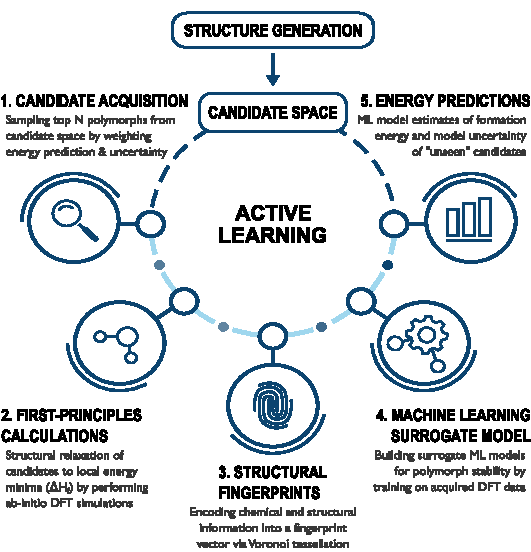
\includegraphics{02_figures/al_diagram/Active_learning_diagram__v3.pdf}}
\caption{\label{fig:all_diagram}
%
% Probably better to keep this caption really concise and refer to the text
Active learning accelerated polymorph discovery algorithm diagram.
%
% , which is constructed through data mining the unique structural motiffs in the OQMD and MP materials databases.
The procedure proceeds through two distinct steps,
first the generation of the hypothetical crystal structure data set (candidate space) and second,
the iterative active learning (AL) algorithm.
%
The AL algorithm proceeds iteratively through:
(1) candidate selection in which a subset of structures in the candidate space are selected based on an acquisition function (in lieu of training data, the initial candidates are randomly sampled),
(2) structural relaxation into local energy minima (formation enthalpy computed),
(3) structure featurization to produce numerical vector for input into ML model,
(4) Machine learning (ML) model training based on acquired structures and \DHf,
(5) Prediction of candidate space's \DHf distribution via ML model.
%
This predicted energy landscape is then used to inform the next generation's acquisition step.
}
\end{figure*}
% __|
% =========================================================


% %%%%%%%%%%%%%%%%%%%%%%%%%%%%%%%%%%%%%%%%%%%%%%%%%%%%%%%%%
% | - Candidate Space Generation
%
% __|
% %%%%%%%%%%%%%%%%%%%%%%%%%%%%%%%%%%%%%%%%%%%%%%%%%%%%%%%%%
% | - PARAGRAPH BODY
%
%The generation of the candidate space is a critical step in the discovery of novel crystal structures for a given system,
%since the initial candidate pool determines which structures that can ultimately be discovered, it is imperative to construct candidates that are sufficiently diverse, such that they encompass as much of the structural diversity in the PES as possible.
%
% TODO PENDING Ask @Ankit for these numbers
% The MP project number should be correct, but the OQMD number might be wrong
% MP{AB2: 2424, AB3: 2341} | OQMD{AB2: 4736, AB3: 28883}
The candidate structure datasets for \IrOtwo and \IrOthree were constructed by first obtaining all \ABtwo and \ABthree structures in the Materials Project\cite{Jain2013} and OQMD\cite{Kirklin2015} databases
(in total \num{4528} \ABtwo and \num{23764} \ABthree entries).
%
To reduce the size of the candidate space while maintaining maximum structural diversity, structurally redundant systems were removed via a space group based structural classification scheme developed by Jain \latin{et al.} \cite{Jain2018}.
%
In short, a material's structural identity is defined by a unique combination of the element-nonspecific stoichiometry (\ABtwo, \ABthree, etc.), space group symmetry and Wyckoff positions, and are referred to as a materials structural prototype.
%
% This is my attempt to further clarify the previous sentence
Materials that share these properties are considered to be structurally identical.
%
For example, the \num{300000} entry dataset of \ABOthree style perovskites in OQMD, which only differ by the choice of elements for A, B, and C, all belong to the same structural prototype, and are thus structurally equivalent.
%
Eliminating these redundant systems from the materials databases reduces the number of entries to \num{697} and \num{259} unique structures for the \ABtwo and \ABthree stoichiometries, respectively.
%
% The orders of magnitude reduction between all structures and unique structures highlights the lack of structural diversity in the OQMD and MP databases.
This reduction leads to orders of magnitude reduction of the search space, as opposed to full utilization of the OQMD and Materials Project databases.
%
Finally, only structures containing $\leq\num{75}$ atoms
(\num{566} and \num{256} \ABtwo and \ABthree structures respectively)
were included to the reduce the computational expense of subsequent DFT calculations.
%
We next substituted iridium and oxygen for the A and B sites, and these Ir-O adapted polymorphs were isotropically relaxed to accommodate their atomic radii.
%
A full bulk DFT optimization recipe was performed on these systems,
yielding a data set of \num{714} relaxed bulk \IrOx polymorphs
(\num{487} and \num{248} structures for \IrOtwo and \IrOthree, respectively),
after discarding \mytilde100 non-converged structures.
%
While not particularly large, our candidate space's size allows us to tractably compute all DFT optimized structures, thus allowing us to benchmark the performance of our methodology.
%
The full details of the candidate space generation and DFT calculations are in the Supplementary Information.
% __|
%%%%%%%%%%%%%%%%%%%%%%%%%%%%%%%%%%%%%%%%%%%%%%%%%%%%%%%%%%%


% %%%%%%%%%%%%%%%%%%%%%%%%%%%%%%%%%%%%%%%%%%%%%%%%%%%%%%%%%
% | - Featurization Strategy
% Short paragraph on Voronoi featurization
% __|
% %%%%%%%%%%%%%%%%%%%%%%%%%%%%%%%%%%%%%%%%%%%%%%%%%%%%%%%%%
% | - PARAGRAPH BODY
%
The active learning algorithm proceeds through a structure featurization scheme based on Voronoi tessellation developed by Ward \latin{et al.} \cite{Ward2017} which produces a \num{271}-length fingerprint vector that is invariant to isotropic lattice changes and somewhat insensitive to the precise atomic coordinates.
%
These fingerprints encode both chemical and structural information by constructing attributes from elemental properties which are weighted by the local environment of the structure via the construction of the Wigner-Seitz cell.
\cite{Wigner1933}
%
Since our AL framework focuses on fixed compositions, the dimensionality of the features are reduced to \num{101} non-zero variance features.
%
% TODO Create cross-validation plot
We further reduce the dimensionality if this set to 10 features via principal component analysis (PCA)~\cite{Tipping1999},
which we found to capture 80\% of the variance in the original feature set while also demonstrating an optimal cross-validation mean absolute error (MAE) (see Figure \ref{fig:cv_anal}).
%
% Further dimensionality reduction was achieved via a principle component analysis (PCA) \cite{Tipping1999}, which was used to reduce the remaining \num{101} fingerprints to \num{10}.
%
% \num{10} PCA components demonstrated the optimal cross-validation mean absolute error (MAE), although only capturing 80\% of the fingerprint's variance (see \ref{fig:cv_anal}).
% __|
%%%%%%%%%%%%%%%%%%%%%%%%%%%%%%%%%%%%%%%%%%%%%%%%%%%%%%%%%%%


% %%%%%%%%%%%%%%%%%%%%%%%%%%%%%%%%%%%%%%%%%%%%%%%%%%%%%%%%%
% | - PARAGRAPH HEADER
% Active Learning Loop
%
% NOTE This paragraph is a bit long, find way to split into 2
% __|
% %%%%%%%%%%%%%%%%%%%%%%%%%%%%%%%%%%%%%%%%%%%%%%%%%%%%%%%%%
% | - PARAGRAPH BODY
%
The active learning algorithm proceeds through iterative generations of ML training, prediction, and acquisition steps that are visualized in Figure~\ref{fig:all_diagram}.
%
% COMBAK Did I get all of the important features of GP here? @Jose
To meet our primary goal of being able to explore and identify the most stable polymorphs within the candidate space,
we construct the AL framework to be
(i) flexible and responsive in improving itself by learning from small batches of newly acquired DFT data,
and (ii) aware of limitations in its surrogate model by incorporating uncertainty estimates into the acquisition decision criteria.
%
GP regressors naturally satisfy both requirements,
and hence we use them with an RBF kernel as implemented in CatLearn.
\cite{hansen2019atomistic,CatLearn_Repo}
%
% NOTE I've introduced the aquis. crit. with the GP uncertainty before talking about aquis. in more detail, need to restructure
%
In the initial generation (generation 0), the model is trained on a set of randomly sampled candidates (unbiased sampling),
and is then used to predict the formation enthalpy (\DHf) of all structures in the candidate space.
%
This predicted energy landscape is then used to choose the next systems to acquire (calculate via DFT) by selecting systems that minimize the GP-LCB (Gaussian process lower confidence bound) acquisition function,
$U = \mu - \kappa \sigma$~\cite{Cox1992}.
%
Here, $\mu$ and $\sigma$ are the predicted \DHf mean and uncertainty, respectively,
and $\kappa$ is a parameter that weights exploitation vs exploration of the search-space (set to 1).
%
At every generation of the AL loop, $N$ structures that minimize the acquisition function are acquired for DFT optimization and are subsequently added to the training data set, where $N$ is AL bin size (here set to 5).
%
% TODO N is used into mean number of atoms (FIX)
The value of $N$, in effect, determines the degree of parallelization of the routine.
%
% The optimal value of $N$ depends on the computational resources available, as small values can result in slow down the discovery rate of the AL algorithm,
% as every DFT calculation needs to be performed more serially.
%
% TODO: Is this statement true?
% Larger values of $N$ speed up the active-learning algorithm, but leads to a higher number of DFT calculations performed before convergence.
%
% COMBAK We are discussing alternative convergence criteria, or whether to even have convergence criteria here
% I think this is fine, just mention a few possible convergence criteria and leave at that
In practice, the AL algorithm proceeds until no more stable polymorphs are found, or after the allocated computational budget is exhausted.
% convergence is achieved, which here is chosen to be the generation at which the structures within the range of metastability, here taken as \num{0.1} eV/atom, are unchanging over three consecutive generations.
% __|
%%%%%%%%%%%%%%%%%%%%%%%%%%%%%%%%%%%%%%%%%%%%%%%%%%%%%%%%%%%


% %%%%%%%%%%%%%%%%%%%%%%%%%%%%%%%%%%%%%%%%%%%%%%%%%%%%%%%%%
% | - Duplicate Structure Removal
%
% __|
% %%%%%%%%%%%%%%%%%%%%%%%%%%%%%%%%%%%%%%%%%%%%%%%%%%%%%%%%%
% | - PARAGRAPH BODY
%
Although initially unique, the structures in the candidate set often relax into one another over the course of the DFT optimization, introducing duplicates in the post-DFT structures.
%
The duplicates are removed, on the fly, during each generation of the AL algorithm
by using the structure similarity quantification method of Su \latin{et al.}~\cite{Su2017}.
%
% The coordination characterization function (CCF) based methodology to quantify the similarity between structures was used to identify and remove duplicate structures.\cite{Su2017}
% __|
%%%%%%%%%%%%%%%%%%%%%%%%%%%%%%%%%%%%%%%%%%%%%%%%%%%%%%%%%%%


  % - 02.01 | *****************************************************************
  \subsection{II. Application of Active Learning to the discovery of stable Ir-O polymorphs}
  %%%%%%%%%%%%%%%%%%%%%%%%%%%%%%%%%%%%%%%%%%%%%%%%%%%%%%%%%%%%%%%%%%%%%%%%%%%%%%%
%% Active Learning Machine Learning Results
%%
%%%%%%%%%%%%%%%%%%%%%%%%%%%%%%%%%%%%%%%%%%%%%%%%%%%%%%%%%%%%%%%%%%%%%%%%%%%%%%%


% #############################################################################
% #############################################################################
% ██████  ███████ ███████ ██    ██ ██   ████████ ███████
% ██   ██ ██      ██      ██    ██ ██      ██    ██
% ██████  █████   ███████ ██    ██ ██      ██    ███████
% ██   ██ ██           ██ ██    ██ ██      ██         ██
% ██   ██ ███████ ███████  ██████  ███████ ██    ███████
% #############################################################################
% #############################################################################
% Notes:
%   - QUESTION Is there any physical intuition that we can gleam from the fingerprints?
%   - QUESTION What did @Chris mean by this? "Computed amorphous phase to define synthesizability"
% #############################################################################
% #############################################################################



% ################################# Paragraph #################################
% %%%%%%%%%%%%%%%%%%%%%%%%%%%%%%%%%%%%%%%%%%%%%%%%%%%%%%%%%%%%%%%%%%%%%%%%%%%%%
% Intro/transition paragraph
%
% %%%%%%%%%%%%%%%%%%%%%%%%%%%%%%%%%%%%%%%%%%%%%%%%%%%%%%%%%%%%%%%%%%%%%%%%%%%%%
% | - Paragraph start
%
We now turn our attention of the application of this active learning scheme to the discovery of stable forms of IrO2 and IrO3.
% Comment on this line | TODO do stuff
%The AL algorithm is applied separately to IrO2 and IrO3 because we are specifically interested in the most stable polymorphs at each stoichiometry.
% TODO How many features drop out when you constrain the stoich.?
%This has an the added benefit of reducing the number of fingerprint vectors from the Voronoi tesselation dramatically (from TEMP to TEMP) because many features are senstive to changes in stoicheometry.
% __|

% ################################# Paragraph #################################
% %%%%%%%%%%%%%%%%%%%%%%%%%%%%%%%%%%%%%%%%%%%%%%%%%%%%%%%%%%%%%%%%%%%%%%%%%%%%%
% Results for IrO3
% MAIN RESULTS:
%   How many generations to find top 2-3 structures?
% We need to call them something else than "convergence plots" (bad name)
% %%%%%%%%%%%%%%%%%%%%%%%%%%%%%%%%%%%%%%%%%%%%%%%%%%%%%%%%%%%%%%%%%%%%%%%%%%%%%
% | - Paragraph start
%
Figure \ref{fig:iro2_al} a and b shows several iterations of the active learning loop for the IrO3 candidate space.
%
The figures plot the predicted (small circles) and aquired (large red-bordered circles) formation energies against the candidate space, sorted by the formation energy.
%
An acquisition bin size of 10 DFT calculations per iteration and an initial seed of 11 calculations were used.
%plots of the AL predictions on the candidate space at particular generations of the AL algorithm for the IrO3 candidate space with an aquisition bin size of 10 DFT calculations per iteration and an initial 11 calculations used for seeding.
%
Figure \ref{fig:iro2_al} a. shows the progression of the model at selected generations of the active learning loop, starting and ending with the initillay seeded generation and final generation, respectivelly.
%
As the ALL aquires more DFT calculations, the predicted uncertainty on the remaining candidate space decreases,
as evidenced by the shrinking error bars with increasing AL generation.
% As seen from Figure\ref{fig:iro2_al} a) the early iterations, where the training data is sparse 
%
The middle panel corresponds to the converged generation of the ALL, which finished after TEMP iterations of the ALL (TEMP DFT calculations).
%
The middle panel is reproduced in figure \ref{fig:iro2_al}, which also shows the real DFT energies accompanying each predicted formation energy (hollow diamonds).
% Probably remove the diamonds and add the parity subplot?
% Figure \ref{fig:iro2_al} b. shows the formation energy, either predicted (small colored circles) or computed (large red-bordered circles), is plotted on the y-axis against all structures in the candidate space of IrO3 polymorphs.
%
It is evident from figure \ref{fig:iro2_al}, that the Gaussian process model is doing a poor job of predicting the DFT formation energy of the candidate space, with an exceptionally poor MAE of ~0.5 eV/atom at the AL generation shown here.
%
This is clearly seen in the parity plot (Fig TEMP), which shows that the predicted DFT energies become increasingly less accurate as stability of the polymorph decreases, with low stability structures tending to reconfigure into lower energy states.
%
This is significantly lower than the leave-one out cross validation error of ~0.15 eV/atom, which is performed by predicting only on optimized strctures, indicating that the issue does not lie with a poor predictive model, but instead with the large degree of structural reorganization that occurs over the course of a typical DFT ionic optimization.
%
This
% TODO Change wording when @Kirsten uses the protosearch to optimize candidates
% UPDATE | Using protosearch pre-optimizer isn't worth it, no siginificant improvement
%Because the candidate space structures are generated
% To compare the performance of the AL routine we compare against a
%
Figure subplot TEMP shows the parity plot of the predicted DFT energies using the fingerprints corresponding to the unoptimized structures (COLOR1) and post-DFT relaxed structures (COLOR2),
plotted against the final post-optimization DFT formation energy.
% Sentence that explains the parity plot
It is clear that the GP model severely underpredicts the energy of the candidate space, especially for systems with less stable predicted formation energies, when predicting onto the candidate space of unoptimized structures (MAE of ~0.5 eV/atom).
%
This is due to the fact that the structures undergo through a large degree of structural rearrangement over the course of the DFT relaxation.
%
Alternatively, the MAE is much lower when the model predicts onto the post-optimized structures (MAE ~0.15 eV/atom),
demonstrating that the poor preditive capabilities is due primarily to structural drift and not to the poor predictive capabilities of the GP model.
%
Despite these shortcomings, figure TEMP (TEMP performance plot) tracks the number of high stability materials (lowest N structures) discovered as a function of the number of DFT calculations for the case of 1.) AL with UCB acquisition function and 2.) AL with a random acquisition function.
%
The random acquisition function emulates the behavior of regression model which exhibits no correlation between the input and output space.
%
Clearly, the rate of discovery for case 1.) is superior to that of case 2.), with our methodology discovering half of the lowest N structures after only TEMP DFT calculations compared to TEMP when acquiring randomley within the candidate space.
% __|


% | - Figure | IrO3 Convergence Plot
\begin{figure*}
\centering
\makebox[\textwidth][c]{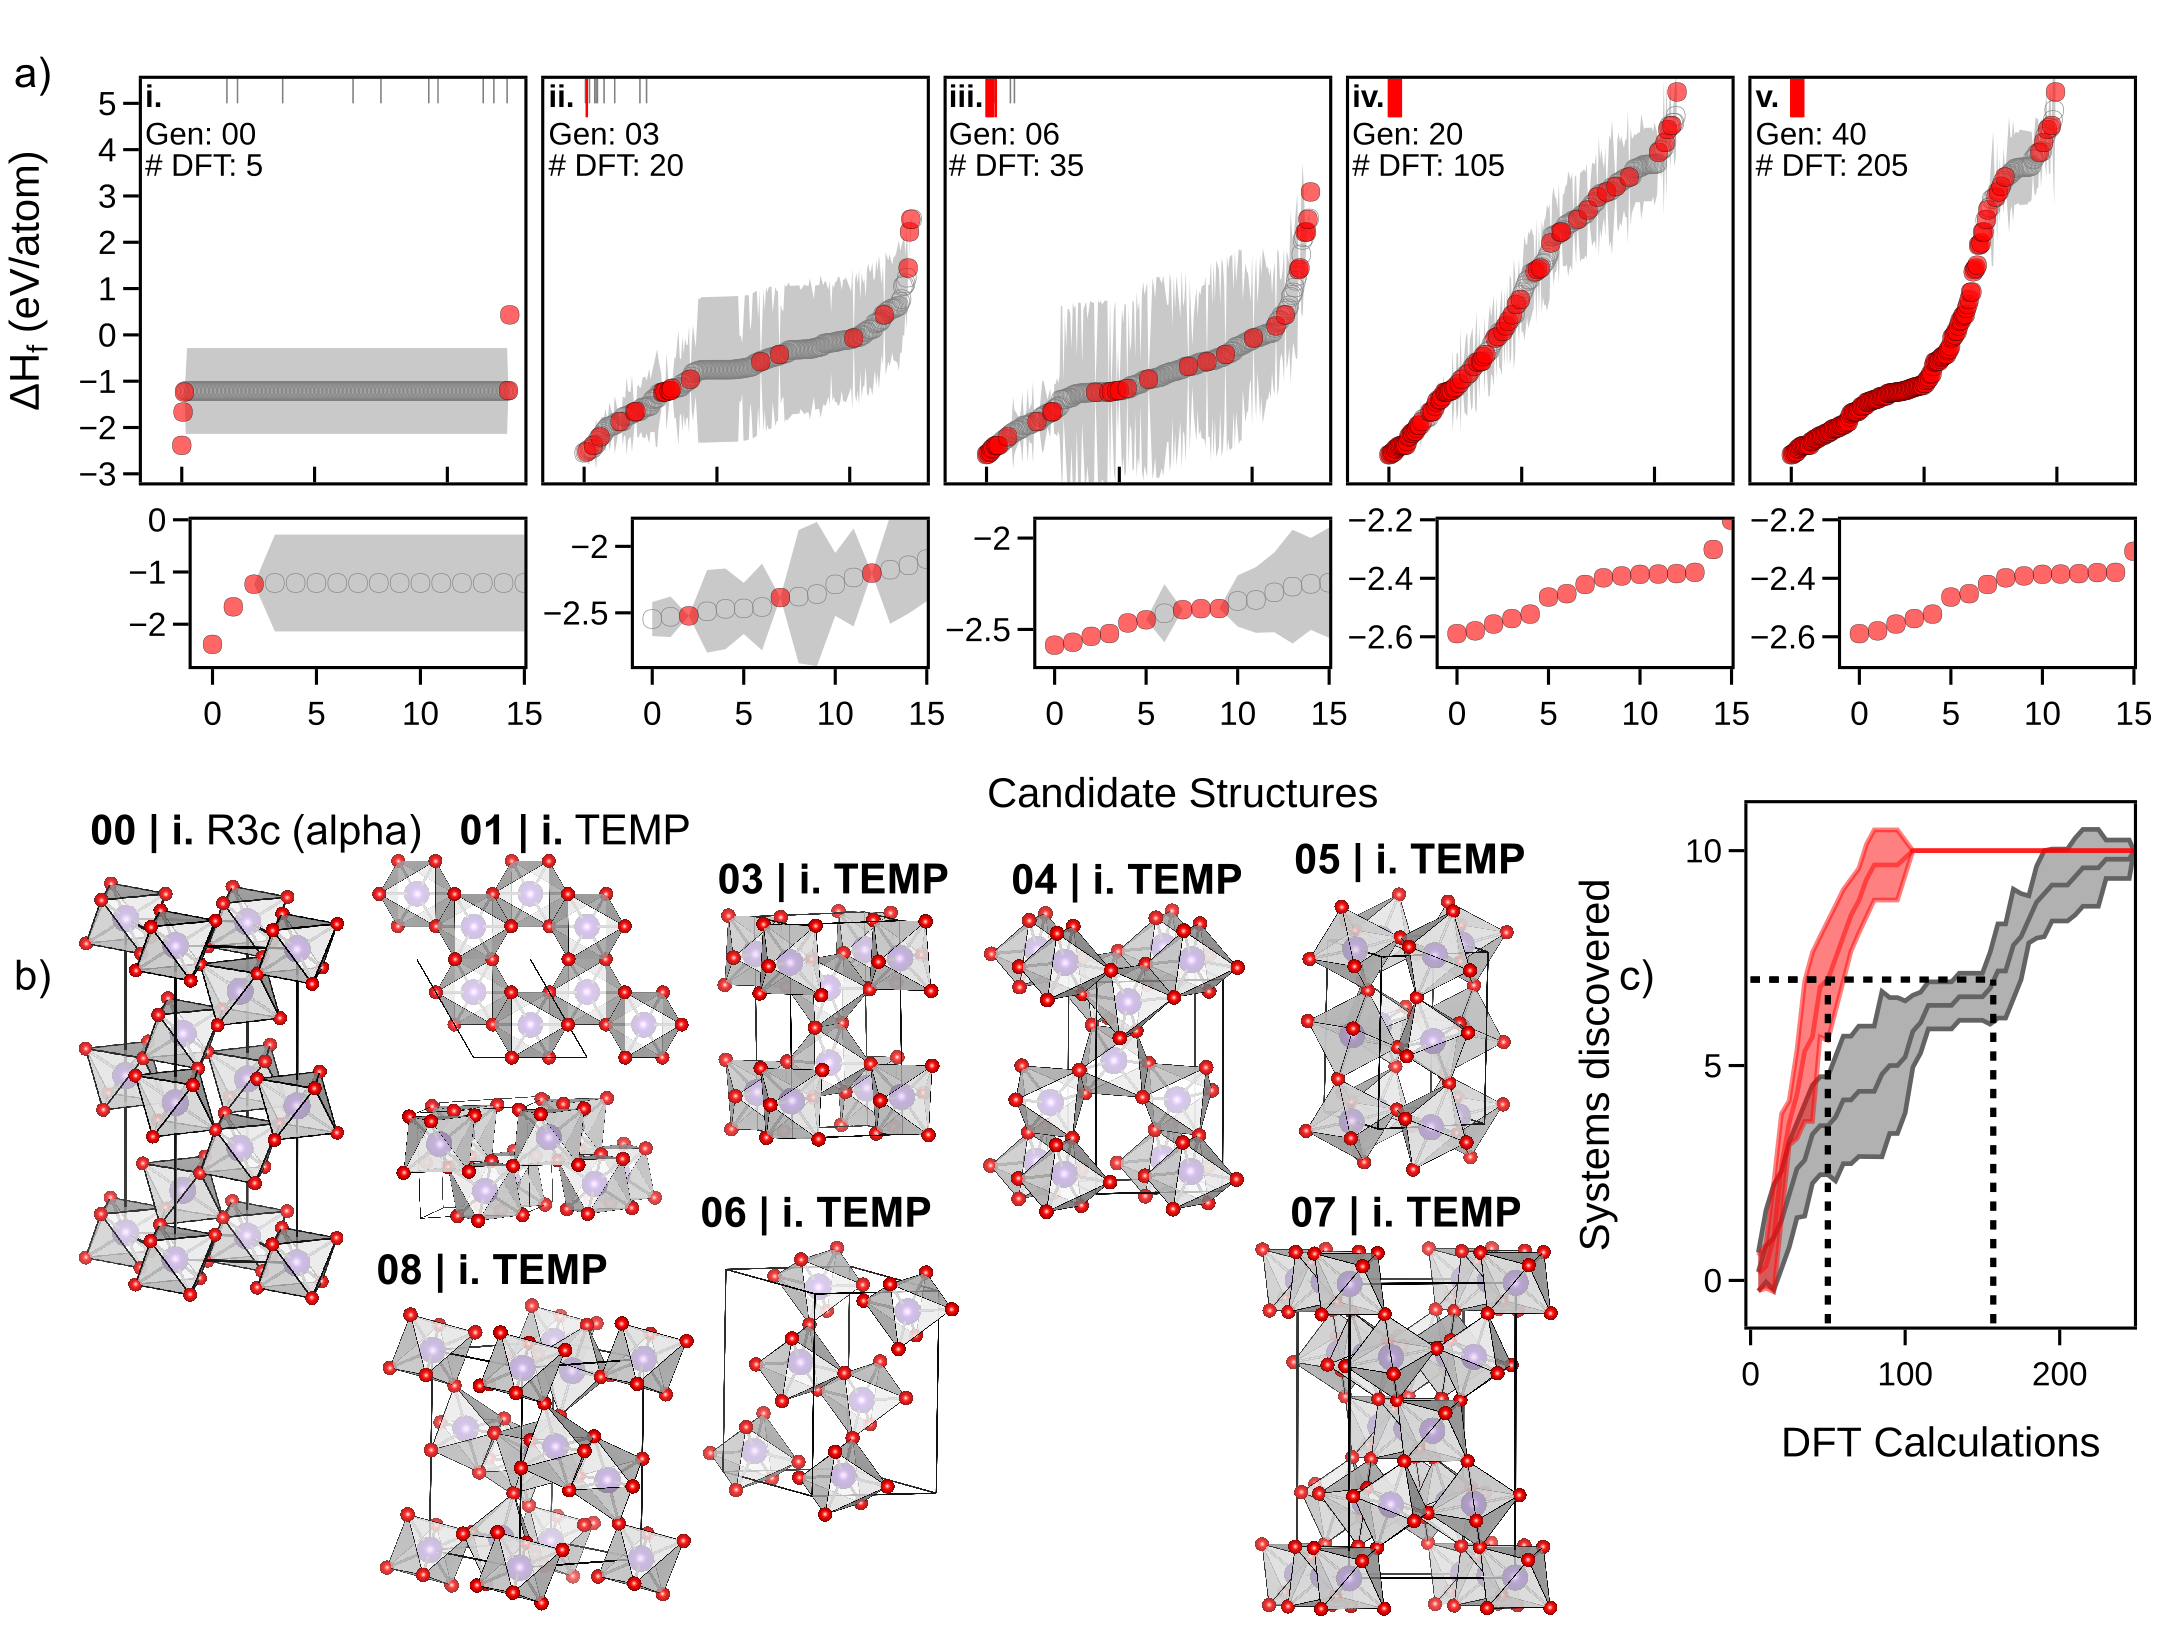
\includegraphics[width=\textwidth,height=\textheight,keepaspectratio]
{02_figures/ml_convergence_plots/test_iro3_al.png}
}
\caption{\label{fig:iro2_al}
Results from machine-learning accelerated active learning material discovery algorithm.
% FORMATION ENTHALPY, FIX
Both (a) and (b) plot the formation enthalpy (either predicted from the model or computed by DFT) for each system in the candidate pool, ordered by decreasing stability (low to high formation energy).
%
Formation energies predicted by the surrogate model are represented by smaller circles,
while acquired DFT formation energies are shown as enlarged red bordered circles.
%
Each data point is colored based on the ordering of the DFT formation energies, with low formation energy systems on the dark end of the spectrum and the highest formation energy species colored light.
%
Error bars representing 1 sigma standard deviation from the Gaussian Process model are shown for each prediction.
%
(a) Series of ML convergence plots at different generations of the active learning algorithm.
%
The middle panel indicates the generation which satisifies the AL stop criteria (see text)
%
(b) Expanded ML plot for the generation that satisfies the stop criteria.
%
Black diamonds indicate the actual DFT formation energy for each system.
%
Inset shows the most stable 20 systems that are within the energetic window of meta-stability (indicated by grey band).
%
(c)
Number of the top 20 polymorphs discovered as a function of the AL generation number for the AL loop using the aquisition criteria in equation TEMP and a control run that utilized a random  aquisition method.


% | - __old__
% Gaussian process machine learning models trained initially on (a) publicly available DFT data for IrO2 and (b) all of the acquired DFT calculations from the active learning algorithm.
% See SI for additional panels at intermediate iterations of the active learning algorithm.
% The Gibbs formation energy (either DFT derived or predicted from the GP model) and associated GP estimated error (2 sigmas or something TEMP) is plotted for each polymorph in the IrO2 candidate space.
% The data points in each subset are ordered from most to least stable (lowest to largest DE formation).
% The individual markers are colored based on their ordering in the final converged GP model.
% Acquired structures are identified by their red borders and slightly larger size.
% The insets show the most stable TEMP structures, where several well known crystal structures are labeled.
% __|

}
\end{figure*}
% __|


  % - 02.02 | *****************************************************************
  \subsection{III. Crystal coordination analysis of discovered phases}
  %%%%%%%%%%%%%%%%%%%%%%%%%%%%%%%%%%%%%%%%%%%%%%%%%%%%%%%%%%%%%%%%%%%%%%%%%%%%%%%
%% Structural analysis of IrO2 and IrO3 oxides
%% NOTES:
%%   - Describe convex hull, classes of structures (\ce{$\alpha$-AlF3} like, rutile like, and layered, should be segregated in hull plot)
%%   - Briefly describe structures within each class, cite in literature where appropriate
%%%%%%%%%%%%%%%%%%%%%%%%%%%%%%%%%%%%%%%%%%%%%%%%%%%%%%%%%%%%%%%%%%%%%%%%%%%%%%%


% ################################# Paragraph #################################
% %%%%%%%%%%%%%%%%%%%%%%%%%%%%%%%%%%%%%%%%%%%%%%%%%%%%%%%%%%%%%%%%%%%%%%%%%%%%%
% TEMP
% %%%%%%%%%%%%%%%%%%%%%%%%%%%%%%%%%%%%%%%%%%%%%%%%%%%%%%%%%%%%%%%%%%%%%%%%%%%%%
% | - Paragraph start\
{\bf There should be a paragraph which discussed the structural drifft and perfromance/acceleration in more detail}
I would use the updated version of Figure 2c. 


Next, we describe the structural variety that is present in our data set of ~1000 IrO2 and IrO3 polymorphs.
% Looks like I wasn't using the algorithm implemented in R52 (David Waroquiers)
The coordination environment package ChemEnv, developed by Waroquiers et. al. \cite{Waroquiers2017} and implemented in pymatgen \cite{Ong2013},was used to assign M-O crystal filed coordination types (e.g. octahedral, square pyramidal, cubic, etc.) to each of the $~$1K structures in our combimed data set.
{\bf Describe in two paragraphs what is shown in Figure 3 and in what the main consequneces of these results}

%
Additional esoteric coordination environments were identified manually, see SI.
% COMBAK What normalization methodd do I end up using for the E and V?
The resulting distribution is included in figure TEMP, which plots the electronic energy and volume, both normalized on a per atom basis
% __|


% | - Figure | Energy vs Volume (motiff distribution)
\begin{figure*}
\centering
\makebox[\textwidth][c]{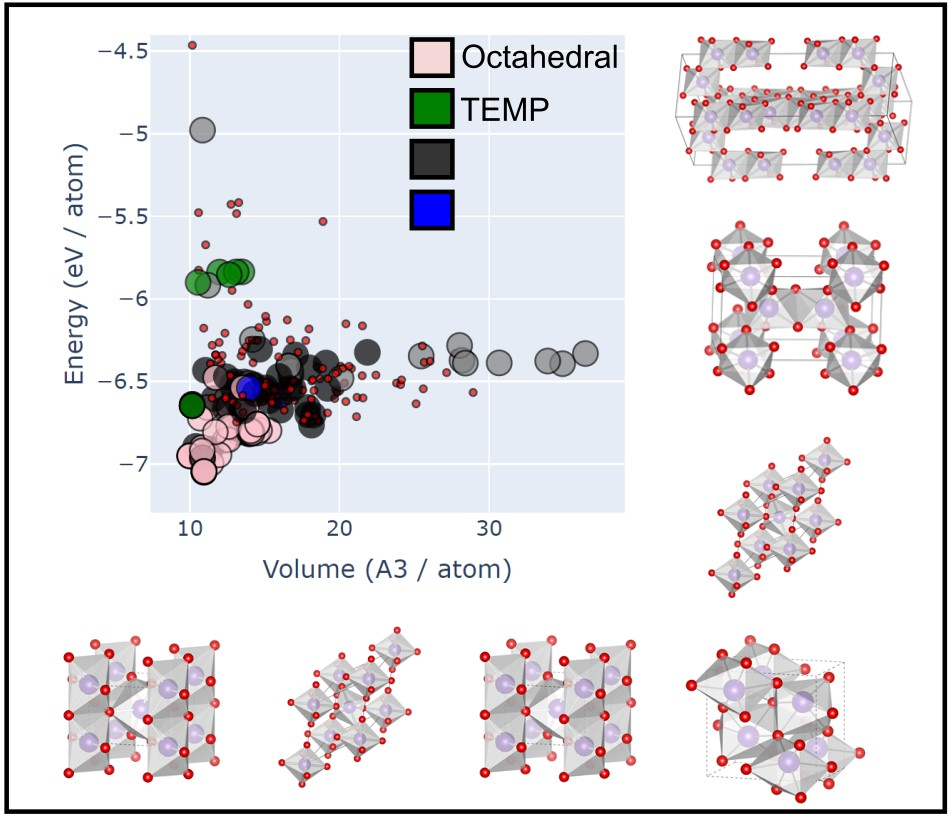
\includegraphics[
width=\textwidth,height=\textheight,keepaspectratio]
{02_figures/e_vs_v_motiffs.jpg}
}
\caption{\label{fig:iro2_al}
% Make sure to update x-axis quantity (volume per atom, Ir, or density, etc.)
Enthalpy of formation for the TEMP|num-iro2-dft IrO2 (circles) and TEMP|num-iro3-dft IrO3 (crosses) structures in the candidate data set plotted against the volume per atom.
%
Color overlays indicate the dominant coordination motiffs as indicated by the legend.
%
Select polymorphs systems are displayed around the plot area.
}
\end{figure*}
% __|






% | - __old__

% | - Figure | IrO2 Convergence Plot
% \begin{figure*}
% \centering
% \makebox[\textwidth][c]{\includegraphics
%   {02_figures/ml_convergence_plots/00_master__iro2-ml-conv_v1__200dpi__0__outplot.png}
%   % {02_figures/ml_convergence_plots/iro2_ml_conv.png}
%   }
% \caption{\label{fig:convergence_plot_iro2_0}
% % #COMBAK Subscript IrO2
% Gaussian process machine learning models trained initially on (a) publicly available DFT data for IrO2 and (b) all of the acquired DFT calculations from the active learning algorithm.
% See SI for additional panels at intermediate iterations of the active learning algorithm.
% The Gibbs formation energy (either DFT derived or predicted from the GP model) and associated GP estimated error (2 sigmas or something TEMP) is plotted for each polymorph in the IrO2 candidate space.
% The data points in each subset are ordered from most to least stable (lowest to largest DE formation).
% The individual markers are colored based on their ordering in the final converged GP model.
% Acquired structures are identified by their red borders and slightly larger size.
% The insets show the most stable TEMP structures, where several well known crystal structures are labeled.
% }
% \end{figure*}
% __|

% | - Figure | IrO3 Convergence Plot
% \begin{figure*}
% \centering
% \makebox[\textwidth][c]{\includegraphics
% {02_figures/ml_convergence_plots/00_master__iro3-ml-conv_v6__200dpi__0__outplot.png}
% % {02_figures/ml_convergence_plots/iro3_ml_conv.png}
% }
% \caption{\label{fig:convergence_plot_iro3_0}
% TEMP.
% }
% \end{figure*}
% __|

% __|


  % - 02.03 | *****************************************************************
  \subsection{III. Electrochemical OER Application}
  % %%%%%%%%%%%%%%%%%%%%%%%%%%%%%%%%%%%%%%%%%%%%%%%%%%%%%%%%%
% | - Electrochemical OER Application
% %%%%%%%%%%%%%%%%%%%%%%%%%%%%%%%%%%%%%%%%%%%%%%%%%%%%%%%%%
%
% OER DFT modelling references:
%   * Man2011
% __|
% %%%%%%%%%%%%%%%%%%%%%%%%%%%%%%%%%%%%%%%%%%%%%%%%%%%%%%%%%



% %%%%%%%%%%%%%%%%%%%%%%%%%%%%%%%%%%%%%%%%%%%%%%%%%%%%%%%%%
% | - Short Intro EChem Section
%
% __|
% %%%%%%%%%%%%%%%%%%%%%%%%%%%%%%%%%%%%%%%%%%%%%%%%%%%%%%%%%
% | - PARAGRAPH BODY
%
% TODO In the previous sections make sure to highlight the alpha and rutile IrO3 phases explicitely so that this sentence makes sense here.
We next performed \latin{ab-initio} thermodynamic simulations to elucidate the electrochemical operational stability of \IrOx and the oxygen evolution reaction (OER) activity of various \IrOthree phases previously computed.
%
In particular, we have decided to compare the stability and activity of the most stable \IrOtwo and \IrOthree polymorphs (rutile and our newly discovered \aIrOthree phase), and the rutile-like \IrOthree polymorph.
%
In addition, we computed the OER activity of a delithiated form of a recently reported $\beta$-Li\textsubscript{x}IrO\textsubscript{3} (referred to here as \bIrOthree) structure, as it is a notable example of a well characterized experimental \IrOthree OER catalyst with exceptional activity.~\cite{Pearce2017,Pearce2019}
% __|
% %%%%%%%%%%%%%%%%%%%%%%%%%%%%%%%%%%%%%%%%%%%%%%%%%%%%%%%%%


% %%%%%%%%%%%%%%%%%%%%%%%%%%%%%%%%%%%%%%%%%%%%%%%%%%%%%%%%%
% | - Bulk Pourbaix Diagram
%
% Explain the Ir and IrO[4-] species
% QUESTION Use E or U for potential variable
% __|
% %%%%%%%%%%%%%%%%%%%%%%%%%%%%%%%%%%%%%%%%%%%%%%%%%%%%%%%%%
% | - PARAGRAPH BODY
%
The bulk Pourbaix diagram of the Ir-H\textsubscript{2}O system is shown in Figure~\ref{fig:bulk_pourbaix}.
%
The diagram was constructed by considering the equilibrium between with the following species: Ir, \rIrOtwo, \aIrOthree,  \rIrOthree, \bIrOthree, and an aqueous dissolved \ce{IrO^{4-}} species.
%
We utilized a free energy correction scheme to reproduce the experimental free energy of \IrOtwo relative to the \ce{Ir} reference state, see the Supplementary Information for further details.
%
While Ir and \rIrOtwo are most stable at low bias, \aIrOthree becomes the thermodynamically dominant phase under the relevant conditions for the OER (potentials around \mytilde1.23 V vs. RHE and an acidic environment)
%
% I want to be careful about how I talk about the metastable structures in the bulk Pourbaix, they strictly speaking shouldn't be there at all
The stability regions of the metastable \rIrOthree and \bIrOthree phases (In the absence of any other \IrOthree polymorph) are indicated by unfilled solid lines, and show that these phases also have a large stability window relative to \IrOtwo and the Ir ion.
%
There are twenty-one unique \IrOthree polymorphs discovered in our search which have a region of stability in the bulk Pourbaix plot, in the pH window of zero to sixteen.
%
% TODO Create energy table for main bulk systems in SI
% The similar formation energies (see Table \ref{table:oer_table}) for all three \IrOthree species suggest some or all of these \IrOthree phases may be present and are stable under OER conditions.
% __|
% %%%%%%%%%%%%%%%%%%%%%%%%%%%%%%%%%%%%%%%%%%%%%%%%%%%%%%%%%


% =========================================================
% FIGURE ==================================================
% =========================================================
% | - Figure | Bulk Pourbaix Diagram
\begin{figure*}[!htb]
\centering
\makebox[\textwidth][c]{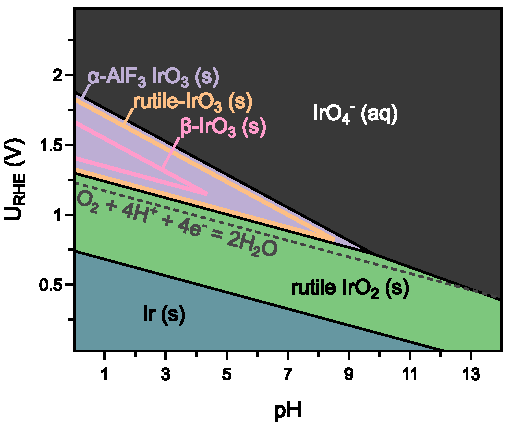
\includegraphics{02_figures/oer_activity_stability/bulk_pourbaix.pdf}}
\caption{\label{fig:bulk_pourbaix}
%
Revised bulk Pourbaix diagram of the \ce{Ir}-\ce{H2O} system as a function of applied potential and pH.
%
The diagram was constructed with Ir(s) (blue), \rIrOtwo (green), various \IrOthree polymorphs and a dissolved \ce{IrO^{4-}} ion species (dark grey).
%
The stability regions corresponding to the metastable \rIrOthree and \bIrOthree polymorphs, in the absence of any competing \IrOthree phase, are displayed as yellow and pink lines, respectively.
%
The thermodynamic onset of OER (water equilibrium at 1.23 V vs. RHE) is also shown.
%
% The most stable system studied (see Table XX in SI for a full list) are Ir-metal Ir(s) (blue), a \rIrOtwo (green), and a dissolved \ce{IrO4[4-]} (grey).
%
% These are compared to the \ce{IrO_3} polymorphs, \aIrOthree (purple), \rIrOthree (orange), and \bIrOthree (pink).
}
\end{figure*}
% __| =====================================================
% =========================================================


% %%%%%%%%%%%%%%%%%%%%%%%%%%%%%%%%%%%%%%%%%%%%%%%%%%%%%%%%%
% | - Introduction to OER Results
%
% __|
% %%%%%%%%%%%%%%%%%%%%%%%%%%%%%%%%%%%%%%%%%%%%%%%%%%%%%%%%%
% | - PARAGRAPH BODY
%
The results of the electrochemical activity and surface stability analysis are summarized in Figure~\ref{fig:oer_volcano}.
%
There, we report the surface energy Pourbaix plots and OER activity for various surface facets at select coverages (*OH, *O, and bare) of the four \IrOx polymorphs from Figure \ref{fig:bulk_pourbaix}.
%
The surface stability Pourbaix plots inform which surface facets and surface coverage species are thermodynamically preferred under OER conditions.
%
This analysis allows us to consider both the stability and activity of particular surface terminations.
%
% TODO Insert XRD simulation into SI and reference here
For each polymorph, surface facets were selected by considering the highest intensity x-ray diffraction peaks from simulated powder-diffraction plots~\cite{Momma2011} (see Figure \ref{fig:xrd_patterns}),
as well as manually selecting high symmetry cleavage planes.
% __|
% %%%%%%%%%%%%%%%%%%%%%%%%%%%%%%%%%%%%%%%%%%%%%%%%%%%%%%%%%


% %%%%%%%%%%%%%%%%%%%%%%%%%%%%%%%%%%%%%%%%%%%%%%%%%%%%%%%%%
% | - Surface Energy Pourbaix Analysis
%
% __|
% %%%%%%%%%%%%%%%%%%%%%%%%%%%%%%%%%%%%%%%%%%%%%%%%%%%%%%%%%
% | - PARAGRAPH BODY
%
Figure~\ref{fig:oer_volcano}a reports the surface energy Pourbaix plots as a function of applied potential (at pH\num{=0}) for the four \IrOx crystals of interest.
%
The bulk phase limits of stability from Figure~\ref{fig:bulk_pourbaix} are included at the bottom of each subplot.
%
For each facet we computed the surface free energy for three coverages, bare, *OH, and *O.
%
At modest overpotentials ($\eta$ \mytilde\num{0.3} or equivalently potentials of \mytilde\num{1.5} V vs. RHE) the convex hull is populated solely by oxygen terminated surfaces.
%
% COMBAK, Revise "mainly" if we include some different coverages
Consequently, we consider mainly oxygen terminated surfaces for the OER analysis.
%
These results are comparable to previous studies on the electrochemical stability of \IrOtwo surfaces~\cite{Nattino2019}, but without considering highly reconstructed facets such as (101).
% __|
% %%%%%%%%%%%%%%%%%%%%%%%%%%%%%%%%%%%%%%%%%%%%%%%%%%%%%%%%%


% =========================================================
% FIGURE ==================================================
% =========================================================
% | - Figure | OER Volcano/Surface Pourbaix
\begin{figure*}
\centering
\makebox[\textwidth][c]{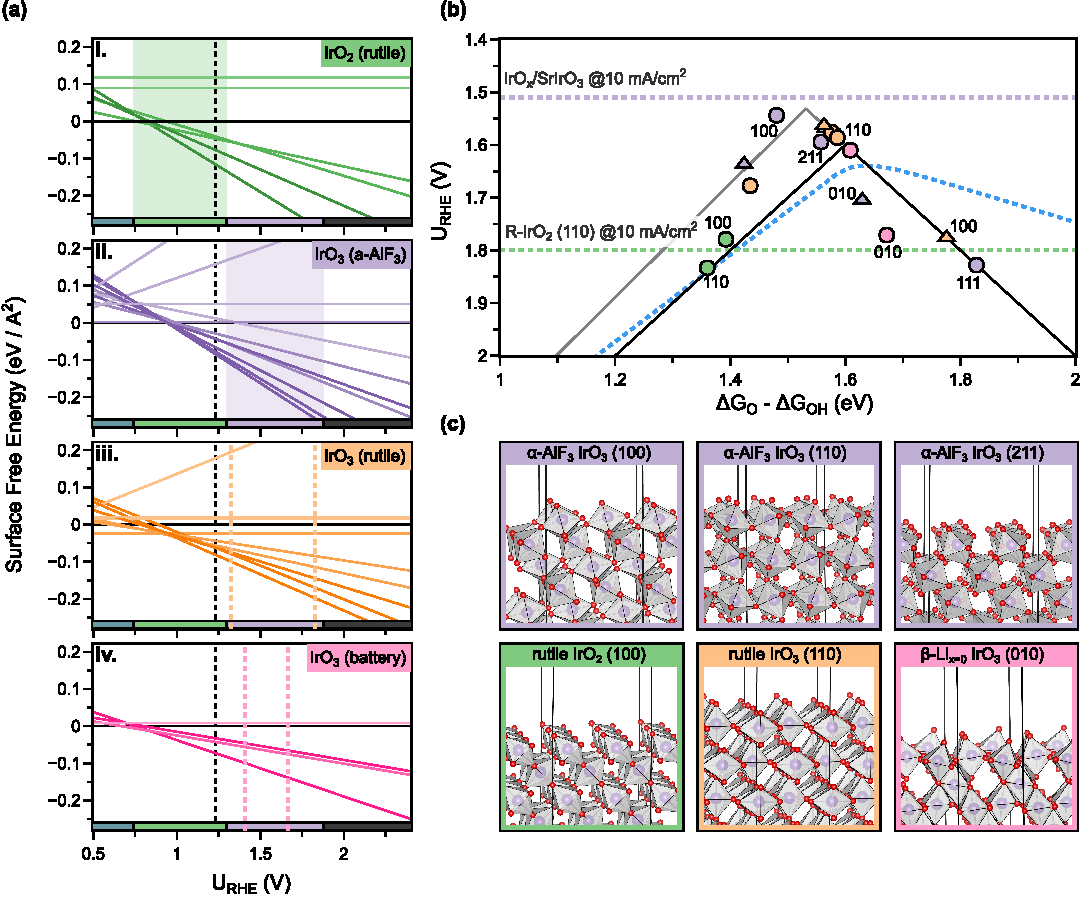
\includegraphics{02_figures/oer_activity_stability/oer_volc_surf_pourb.pdf}}
\caption{\label{fig:oer_volcano}
% TODO Insert green band into figure, insert experimental references for this
%
Summary of OER results for the following four bulk structures of \IrOx: \rIrOtwo (green), \aIrOthree (purple), \rIrOthree (orange), and \bIrOthree (pink).
%
(a) Surface energy Pourbaix diagrams for each structure, with the surface energy of various facets and coverages shown as a function of applied potential (V vs. RHE).
%
Surfaces with coverages of bare surfaces (light lines), *OH covered surfaces (medium lines) and *O terminated surfaces (thick lines) are shown.
%
The bulk Pourbaix diagram's bounds of stability at pH \num{0} are superimposed at the bottom of each subplot.
%
The pseudo-stability regimes for the meta-stable \bIrOthree and \rIrOthree are indicated by dashed vertical lines.
%
(b) OER activity volcano for \IrOx systems considered utilizing the \DGOmOH thermochemical descriptor.
%
% TODO Add citations here
The horizontal lines correspond to recent experimental OER limiting potentials for \IrOtwo and \IrOthree~\cite{Seitz2016}, and were taken at a current density of \num{10} mA cm\textsuperscript{-2}.
% The purple dotted line corresponds to the experimental limiting potential at \num{10} mA cm\textsuperscript{-2} for \ce{IrO_3} \cite{Seitz2016},
% while the green band corresponds to the range of experimentally observed overpotentials for pristine \ce{IrO_2} catalysts as reported in literature.
%
(c) Corresponding structural models for select OER surfaces.
%
% (c) Select surface facets for the four \IrOx crystal systems considered.
%
Color legend: oxygen (red), purple (iridium), coordination motif (white).
}
\end{figure*}
% __| =====================================================
% =========================================================


% %%%%%%%%%%%%%%%%%%%%%%%%%%%%%%%%%%%%%%%%%%%%%%%%%%%%%%%%%
% | - OER Volcano
% TODO We don't mention new old/new scaling volcanos
% __|
% %%%%%%%%%%%%%%%%%%%%%%%%%%%%%%%%%%%%%%%%%%%%%%%%%%%%%%%%%
% | - PARAGRAPH BODY
%
% Replace G_O and G_OH with my custom macros for consistency
The OER activity (in terms of the limiting potential) for select oxygen terminated surfaces are shown in Figure \ref{fig:oer_volcano}b plotted against the \DGOmOH thermodynamic descriptor.
% $\Delta G_\mathrm{O} - \Delta G_\mathrm{OH}$
%
The corresponding surface structures for select systems are visualized in Figure \ref{fig:oer_volcano}c.
%
The \rIrOtwo surfaces bind the OER intermediates relatively strongly,
with theoretical limiting potentials of \mytilde\num{1.8} V vs. RHE (overpotential of 0.57 V vs. RHE) with a *O to *OOH potential limiting step.
%
% Cite Cr-IrO2 paper (ours) and something else here
These results are in agreement with previous experimental, and the latest theoretical studies.
%
The predicted overpotentials of our \rIrOtwo systems are within the range of experimentally observed overpotentials found in literature.
%
% Reference all experimental IrO2 overpotentials I can find
The surfaces of the three \IrOthree polymorphs have \DGOmOH descriptor values shifted to higher energies, indicative of weaker binding energetics (see Figure \ref{fig:scaling_relations}).
% The three \IrOthree polymorph surfaces all have a $\Delta G_\mathrm{O} - \Delta G_\mathrm{OH}$ descriptor towards the top and right of the volcano, indicative of weaker binding energetics.
%
% COMBAK Report just *OH, I have the other ones to
% O: 1.2 eV; *OOH: 1.4 eV
On average, the binding for *OH is weakened by 0.7 eV relative to \IrOtwo.
%
The highest performing systems include the (100), (110), and (211) facets of \aIrOthree, \bIrOthree (101), and \rIrOthree (110).
%
These surfaces have overpotentials of \mytilde\num{0.4} V vs. RHE,
which represents a \mytilde\num{0.2} V vs. RHE improvement over \rIrOtwo.
%
The primary driver for the improved OER activity is the higher oxidation state of \IrOthree compared to \IrOtwo
(\ce{Ir^{6+}} and \ce{Ir^{4+}}, respectively)
%
The more oxygen saturated \IrOthree systems thus bind OER intermediates more weakly, which for overbinding materials like \IrOtwo and \RhOtwo leads to more ideal scaling.
%
The exact improvement in the theoretical overpotential is slightly dependent on the DFT level of theory and the inclusion of spin polarization, and has been discussed recently.~\cite{Seitz2016,Strickler2019}
%
% TODO COMBAK There should be one more sentence about microkinetic volcano
Additionally, we include a micro-kinetic volcano for the OER from recent work by Dickens \latin{et al.}~\cite{Dickens2019},
which plots the potential needed to reach a current density of 10 mA/cm^{2} at a function of the \DGOmOH descriptor.
%
% We note that the computed  overpotentials for our \rIrOtwo system differs from that reported in literature~\cite{Seitz2016} by \mytilde\num{0.2} V.
%
% This discrepancy is due to our inclusion of spin-polarization in our \latin{ab-initio} calculations, which was neglected in Seitz \latin{et al.}.
%
% For further details, we'll refer readers to the SI of a previous publication.\cite{Strickler2019}
% __|
% %%%%%%%%%%%%%%%%%%%%%%%%%%%%%%%%%%%%%%%%%%%%%%%%%%%%%%%%%


% - 03 | Conclusion ***********************************************************
\section{Conclusion}
% %%%%%%%%%%%%%%%%%%%%%%%%%%%%%%%%%%%%%%%%%%%%%%%%%%%%%%%%%
% | - Conclusions
% TEMP
% __|
% %%%%%%%%%%%%%%%%%%%%%%%%%%%%%%%%%%%%%%%%%%%%%%%%%%%%%%%%%


% \textbf{Points our results address that are raised in the intro:}

% %%%%%%%%%%%%%%%%%%%%%%%%%%%%%%%%%%%%%%%%%%%%%%%%%%%%%%%%%
% | - PARAGRAPH HEADER
% Conclusions on AL and results
% __|
% %%%%%%%%%%%%%%%%%%%%%%%%%%%%%%%%%%%%%%%%%%%%%%%%%%%%%%%%%
% | - PARAGRAPH BODY
%
% \textbf{Generation of structurally diverse search space and efficient sampling of it.}
We have described a cogent procedure for generating and searching a structurally diverse candidate space of bulk structural prototypes with a desired composition.
%
Once this space is enumerated, we show how it can can be efficiently searched using an algorithm with an active learning loop without a prior knowledge of accurate atomic positions.
%
In most cases, the DFT optimization of only a fraction of the candidates leads to identification of the most stable polymorphs.
%
In particular, this approach is well-suited for discovery in structurally diverse structures, such as metal oxides and other metal-ligand bulk systems, where there exits a large degree of structural diversity.
%
The current dataset includes octahedral, tetrahedral, square-pyramidal, cubic, and square-planar Ir-O conformers.
%
We also note, that our AL algorithm is capable of discovering experimentally known phases such as pyrite, columbite and layered \IrOtwo and several recently discovered layered \IrOthree phases formed by Li$^+$ deintercalation.
%
In particular, we have identified a number of previously unknown \IrOthree polymorphs below the amorphous synthesizability limit,
including a new globally stable \aIrOthree phase.
%
This high valency Ir$^{6+}$ phase is stable under OER relevant conditions and has an ideal 100\% corner-sharing octahedral structure, a short Ir-O bond length of 1.93 \angstrom, and also has a very high surface coverage of active oxygens.
%
Calculations of surface thermodynamics reveal this structure and other OER stable \IrOthree phases have much higher theoretical OER activity than a benchmark rutile \IrOtwo.
%
The thermodynamic stability and high OER activity of the \aIrOthree phase may provide clues as to the nature of the yet uncharacterized structures reported after reconstruction of \ce{SrIrO_{3}} and \IrOx precursors under OER reaction conditions.
%
Methods combining diverse structural generation, AL-enabled accelerated searches, and \mbox{ab-initio} simulation of material performance could open up new avenues for in silico material design with application tailored structural properties.
% __|
% %%%%%%%%%%%%%%%%%%%%%%%%%%%%%%%%%%%%%%%%%%%%%%%%%%%%%%%%%







% | - __old__

% In conclusion, we have demonstrated an active learning accelerated algorithm for the discovery of stable crystal polymorphs by searching through a candidate space of structurally distinct iridium-oxide phases.
% %
% % TODO Can I generalize this result for both IrO2 and IrO3?
% % TODO Use percentage of total systems instead of just # of DFT calcs
% The algorithm can identify a majority of the most stable polymorphs (7 of the 10 most stable) in a candidate set after only computing a fraction of them via DFT (\mytilde90 DFT optimizations).
% %
% For \IrOtwo, we find confirm the rutile phase as the most stable crystal structure, while also finding several well known phases, including anatase, columbite, as well as several new phases of \IrOtwo.
% %
% For the relatively unexplored \IrOthree we found a new globally stable phase (\aIrOthree), a completely corner sharing octahedral structure with space group 182.
% %
% % Implications for for future studies of polymorphs
% %
% % Describe the level of acceleration achieved, effect of structural drift, implications for future studies
% We have analyzed the local and global structural coordination and revealed that octahedral coordination environments are predominantly preferred, although we also have a large degree of structural diversity in our dataset (octahedral, tetrahedral, square-pyramidal, cubic, and square-planar are all represented)
% %
% % Discuss the differences connectivity/M-O bonds lengths is different between IrO2 and IrO3
% %
% We constructed a revised bulk Pourbaix diagram for Ir-H$_2$O, including the newly found \aIrOthree phase and revealed that \aIrOthree has a substantial window of stability in the OER relevant potentials and pH.


% __|


% #############################################################################
% - Acknowledgment ************************************************************
\begin{acknowledgement}

% COMBAK | Add to, and finalize this
Organizations to acknowledge
TRI
SUNCAT
Stanford
NERSC
etc.

% NOTE | Copied and pasted from some sample text @Michal sent me
JAGT and MB acknowledge the support by the U.S. Department of Energy, Office
of Science, Office of Basic Energy Science, via Grant DE-SC0008685 to the
SUNCAT Center of Interface Science and Catalysis.

The authors would like to acknowledge the use of the computer time allocation
for the “Transition metal-oxide and metal surfaces: applications and
reactivity trends in catalysis” at the National Energy Research Scientific
Computing Center, a DOE Office of Science User Facility supported by the
Office of Science of the U.S. Department of Energy under Contract No.
DE-AC02-05CH11231.

\end{acknowledgement}
% __|
% #############################################################################


% | - Supplementary Information ***********************************************

% | - __latex_setup__
\clearpage
\renewcommand{\thefigure}{S\arabic{figure}}
\setcounter{figure}{0}
\renewcommand{\thetable}{S\arabic{table}}
\setcounter{table}{0}
% __|

\begin{suppinfo}
%%%%%%%%%%%%%%%%%%%%%%%%%%%%%%%%%%%%%%%%%%%%%%%%%%%%%%%%%%%`
%% Supporting Information
%%
%% TODO: Free energy corrections to OER intermediates, OER mechanism
%%%%%%%%%%%%%%%%%%%%%%%%%%%%%%%%%%%%%%%%%%%%%%%%%%%%%%%%%%%


% #########################################################
\section{Active Learning ML Section}  % ###################
% #########################################################
%
% #########################################################
% | - Active Learning ML Section

% %%%%%%%%%%%%%%%%%%%%%%%%%%%%%%%%%%%%%%%%%%%%%%%%%%%%%%%%%
\subsection{Candidate space generation}  % %%%%%%%%%%%%%%%%
% %%%%%%%%%%%%%%%%%%%%%%%%%%%%%%%%%%%%%%%%%%%%%%%%%%%%%%%%%
%
% %%%%%%%%%%%%%%%%%%%%%%%%%%%%%%%%%%%%%%%%%%%%%%%%%%%%%%%%%
% | - Candidate space generation


% %%%%%%%%%%%%%%%%%%%%%%%%%%%%%%%%%%%%%%%%%%%%%%%%%%%%%%%%%
% | - Candidate Generation Intro
% Basic intro into candidate generation
% High-level overview again
%   * Data mining OQMD MP fro AB2/3 entries
%   * Reduce data set by eliminating structurally redundant systems
%     * This is done with Ankit's scheme
% __|
% %%%%%%%%%%%%%%%%%%%%%%%%%%%%%%%%%%%%%%%%%%%%%%%%%%%%%%%%%
% | - PARAGRAPH BODY
%
Here we describe the methodology to construct the set of structural candidates in more detail.
%
The first step of the procedure is to mine materials databases for entries with the desired non-element specific stoichiometry (\latin{i.e.} \ABtwo and \ABthree).
%
Since many of the entries in these databases are structurally redundant,
we used a structure classification scheme to reduce the data set to a structurally unique set.
%
Once this is accomplished, the elements of interest were then substituted into the database structures,
which at this point had their original elemental composition from their database.
%
Finally, the structures are isotropically expanded or contracted to accommodate the difference between the atomic radii of the original elements in the structure and the user defined elements.
%
This procedure of ``pre-optimization'' is an important because it generates reasonable initial geometries which would otherwise produce poor fingerprint representations and lead to a large degree of structural shift during the course of DFT optimization.
% __|
%%%%%%%%%%%%%%%%%%%%%%%%%%%%%%%%%%%%%%%%%%%%%%%%%%%%%%%%%%%


% %%%%%%%%%%%%%%%%%%%%%%%%%%%%%%%%%%%%%%%%%%%%%%%%%%%%%%%%%
% | - TEMP
% Data-mining OQMD and MP
% __|
% %%%%%%%%%%%%%%%%%%%%%%%%%%%%%%%%%%%%%%%%%%%%%%%%%%%%%%%%%
% | - PARAGRAPH BODY
%Herein, we take advantage of the structural diversity already present in materials databases to construct our candidates.
%
We utilized two materials databases, the Open Quantum Materials (OQMD) and the Materials Project (MP) databases because of their large and diverse datasets of crystalline inorganic materials.
%
% TODO Approx. when did Ankit parse these databases
At the time that we originally mined these databases (2018), there were \num{61471} inorganic compounds in the MP database and \num{435583} entries in the OQMD database.
%
We note that the databases have expanded the number of entries considerably since we originally parsed them,
although the number of unique crystal polymorphs is not expected to have increase significantly.
% __|
%%%%%%%%%%%%%%%%%%%%%%%%%%%%%%%%%%%%%%%%%%%%%%%%%%%%%%%%%%%


% %%%%%%%%%%%%%%%%%%%%%%%%%%%%%%%%%%%%%%%%%%%%%%%%%%%%%%%%%
% | - TEMP
%
% __|
% %%%%%%%%%%%%%%%%%%%%%%%%%%%%%%%%%%%%%%%%%%%%%%%%%%%%%%%%%
% | - PARAGRAPH BODY
%
The structural classification scheme of Jain \latin{et al.} was used assign the crystal prototype, consisting of standardized spacegroup and Wyckoff positions, as well as the element-nonspecific stoichiometry of each structure (\num{497054} in total). This prototype designation can serve as a structural fingerprint and has successfully been applied towards the prediction of formation energies of inorganic compounds \cite{Jain2018}.
%
% COMBAK Revise if Ankit's scheme becomes it's own section
% If it's not ready now, let's not include it.
%See section TEMP for more details on the symmetry based structural classification scheme.
%
Once classified, we selected all entries with the desired stoichiometry of \ABtwo and \ABthree,
for which MP has \num{2424} and \num{2341} \ABtwo and \ABthree entries, respectively,
and OQMD has \num{4736} and \num{28883} \ABtwo and \ABthree entries, respectively.
%
The reason that there are considerably more \ABthree compounds in OQMD is due to the extensive compositional permutation of binary alloys in a cubic \ABthree structure.
%
Within each stoichiometry, the structural classification was used to eliminate structurally redundant systems,
\latin{i.e.} systems that share their stoichiometry, space-group, and Wyckoff positions.
%
This process reduces the data set to \num{620} and \num{219} unique structures of \ABtwo and \ABthree for MP and \num{397} and \num{194} structurally unique \ABtwo and \ABthree OQMD entries.
%
Combining the MP and OQMD data sets ultimately results in a dataset of \num{688} \ABtwo and \num{254} \ABthree structurally unique candidates.
% __|
%%%%%%%%%%%%%%%%%%%%%%%%%%%%%%%%%%%%%%%%%%%%%%%%%%%%%%%%%%%


% =========================================================
% TABLE ===================================================
% =========================================================
% | - Table | OQMD MP Structures
\begin{table}[!htb]

  \caption{\label{table:database_structures}
    %
    (a) Number of entries in the OQMD and MP materials databases for the \ABtwo and \ABthree stoichiometries.
    %
    (b) Final number of unique structural candidates for \ABtwo and \ABthree.
    }
  %
  % | - Subtable a
  \begin{subtable}{.5\linewidth}
  \centering
  \caption{}
  %
   %
    %
    \begin{tabular}{cccc}
    \textbf{}         & \textbf{}        & \multicolumn{2}{c}{\textbf{Entries}} \\
    \textbf{Database} & \textbf{Stoich.} & \textbf{Total}   & \textbf{Unique}   \\
    OQMD              &                  & 435,583          &                   \\
                      & \ABtwo           & 4,736            & 397               \\
                      & \ABthree         & 28,883           & 194               \\
    \hline
    MP                &                  & 61,471           &                   \\
                      & \ABtwo           & 2,424            & 620               \\
                      & \ABthree         & 2,341            & 219
    \end{tabular}
    %
   %
  %
  \end{subtable}
  % __|
  %
  %
  \newline
  \vspace*{0.8 cm}
  \newline
  %
  %
  % | - Subtable b
  \begin{subtable}{.5\linewidth}
  \centering
  \caption{}
  %
   %
    %
    \begin{tabular}{cc}
    \multicolumn{2}{c}{\textbf{Final Candidate Set}} \\
    \textbf{Stoich.}   & \textbf{Unique Structures}  \\
    \ABtwo             & 697                         \\
    \ABthree           & 259
    \end{tabular}
    %
   %
  %
  \end{subtable}
  % __|
  %
\end{table}
% __| =====================================================
% =========================================================

% __|


% %%%%%%%%%%%%%%%%%%%%%%%%%%%%%%%%%%%%%%%%%%%%%%%%%%%%%%%%%
\subsection{Structure featurization and data processing}  %
% %%%%%%%%%%%%%%%%%%%%%%%%%%%%%%%%%%%%%%%%%%%%%%%%%%%%%%%%%
%
% %%%%%%%%%%%%%%%%%%%%%%%%%%%%%%%%%%%%%%%%%%%%%%%%%%%%%%%%%
% | - Structure featurization and data processing


% %%%%%%%%%%%%%%%%%%%%%%%%%%%%%%%%%%%%%%%%%%%%%%%%%%%%%%%%%
% | - TEMP
%
% __|
% %%%%%%%%%%%%%%%%%%%%%%%%%%%%%%%%%%%%%%%%%%%%%%%%%%%%%%%%%
% | - PARAGRAPH BODY
%
Structures are featurized using the Voronoi tessellation method developed by Ward et al. \cite{Ward2017}.
%
Zero-variance features that don't encode for any information within a set of structures with constant composition and stoichiometry are removed before model training, reducing the number of feature columns from \num{271} to \num{101}.
%
The number of features are further reduced to \num{10} by performing a principal component analysis (PCA).
%
The optimal number of principle components was found by computing the cross-validation MAE on the post-relaxation fingerprints as a function of PCA components (Figure \ref{fig:cv_anal}),
where it was found that 10 PCA components is sufficient to minimize the error.
% TODO Add all of the feature engineering steps here
% __|
%%%%%%%%%%%%%%%%%%%%%%%%%%%%%%%%%%%%%%%%%%%%%%%%%%%%%%%%%%%


% __|


% =========================================================
% FIGURE ==================================================
% | - Figure | Cross-validation analysis ******************
\begin{figure*}[!htb]
\centering
\makebox[\textwidth][c]{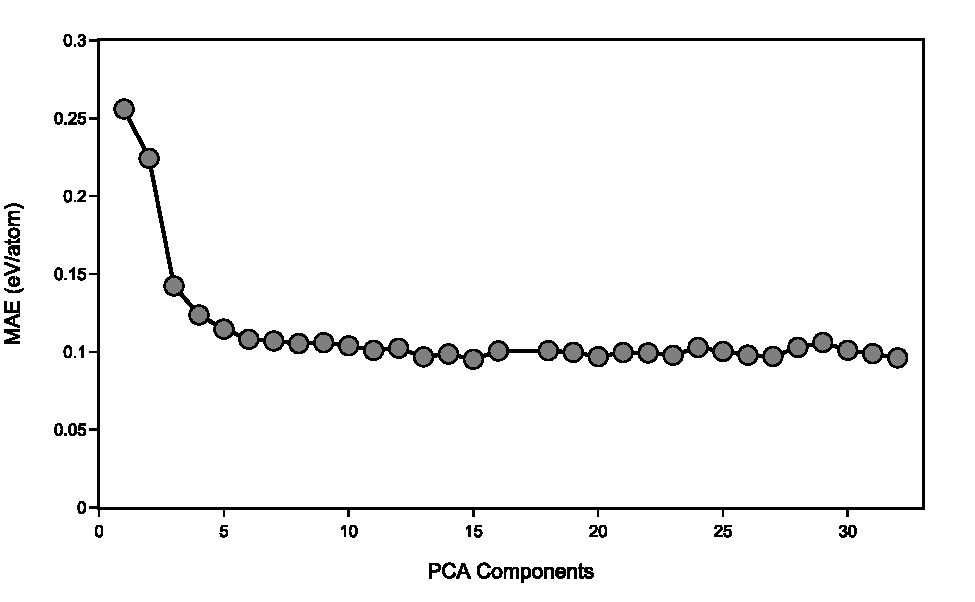
\includegraphics
{02_figures/SI_figures/00_mae_pca_plot__v0.pdf}}
\caption{\label{fig:cv_anal}
20-fold cross validation mean absolute error (MAE) as a function of the number of PCA components used for the GP-regression for \IrOthree.
%
Only post-relaxation fingerprints were used for both training and testing to avoid issues with structural drift.
%
All structural duplicates in the post-relaxation dataset were removed.
}
\end{figure*}
% __|
% =========================================================


% %%%%%%%%%%%%%%%%%%%%%%%%%%%%%%%%%%%%%%%%%%%%%%%%%%%%%%%%%
\subsection{Gaussian process regression model}  % %%%%%%%%%
% %%%%%%%%%%%%%%%%%%%%%%%%%%%%%%%%%%%%%%%%%%%%%%%%%%%%%%%%%
% Relevant details about the ML Gaussian process here
%
% %%%%%%%%%%%%%%%%%%%%%%%%%%%%%%%%%%%%%%%%%%%%%%%%%%%%%%%%%
% | - Gaussian process regression model


% %%%%%%%%%%%%%%%%%%%%%%%%%%%%%%%%%%%%%%%%%%%%%%%%%%%%%%%%%
% | - TEMP
%
% __|
% %%%%%%%%%%%%%%%%%%%%%%%%%%%%%%%%%%%%%%%%%%%%%%%%%%%%%%%%%
% | - PARAGRAPH BODY
%
Gaussian process machine learning regression models were picked due to their highly flexible fits and high performance in situations with small data sets.
%
We utilized the Gaussian Process regression module as implemented in CatLearn.\cite{hansen2019atomistic,CatLearn_Repo}
%
The Gaussian Process recipe we developed utilized two isotropic Gaussian kernels which differ only in the value of the initial length scale parameter, $l$: \textbf{Raul:isn't the scaling optimized for each of them, so that $s$ is also different? Also please add noise kernel in equation below.}

\begin{equation}
    k(x,x') = s_1 exp \Bigl ( \frac{-|x-x'|^2}{2l_1^2}\Bigr) + s_2 exp\Bigl(\frac{-|x-x'|^2}{2l_2^2}\Bigr) + NOISE-kernel?
\end{equation}


Here, isotropic refers to keeping the dimensionality of the kernel equal to one instead of an anisotropic kernel which was found to be difficult to optimize.
%
The first GP kernel was constructed with a length scale parameter of 1 while for the second kernel the length scale was reduced by a factor of ten (0.1). This was done with the aim of producing a model that is responsive to both long- and short-range features in the input space.
%
Additionally, the noise parameter, $TEMP$, was set to a value of \num{0.025}, the scaling parameters, $s_1$, $s_2$ and $\alpha$ was set to 5.2.
%
% TODO Double check that I said it correctly, might be minimizing the LML
These initial value for the hyper-parameters of the GP kernel are then optimized during every training round,
which occurs once per active learning loop,
and is done by maximizing the log marginal likelihood of the model and training data.
% __|
%%%%%%%%%%%%%%%%%%%%%%%%%%%%%%%%%%%%%%%%%%%%%%%%%%%%%%%%%%%





% __|


% %%%%%%%%%%%%%%%%%%%%%%%%%%%%%%%%%%%%%%%%%%%%%%%%%%%%%%%%%
\subsection{Bulk polymorph DFT optimization}  % %%%%%%%%%%%
% %%%%%%%%%%%%%%%%%%%%%%%%%%%%%%%%%%%%%%%%%%%%%%%%%%%%%%%%%
% VASP
% PBE exchange correlation functional
% spin-polarized calculations
% plane-wave cutoff of 600 eV
% %%%%%%%%%%%%%%%%%%%%%%%%%%%%%%%%%%%%%%%%%%%%%%%%%%%%%%%%%
% | - Bulk polymorph DFT optimization


% %%%%%%%%%%%%%%%%%%%%%%%%%%%%%%%%%%%%%%%%%%%%%%%%%%%%%%%%%
% | - TEMP
%
% __|
% %%%%%%%%%%%%%%%%%%%%%%%%%%%%%%%%%%%%%%%%%%%%%%%%%%%%%%%%%
% | - PARAGRAPH BODY
%
All DFT calculations were performed using density functional theory (DFT) implemented via the Vienna \latin{ab-initio} simulation package (VASP) \cite{Kresse1995,Kresse1996_0,Kresse1996_1} and utilizing the PBE exchange-correlation functional\cite{Perdew1996}.
%
A cutoff plane-wave cutoff of 600 eV was used, and calculations were spin-polarized.
%
A variable k-point mesh was used such that a k-point density of at least \num{20} k-points per reciprocal space dimension.
%
All bulk systems were run through the following computational recipe to converge the equilibrium structure, with \num{3} distinct phases.
%
structures are only advanced to the next phase when the previous phase completes without error.
\\
1. An ISIF \num{7} calculation to optimize only the volume (initial volume of cell may be really off).
\\
2. Three consecutive ISIF \num{3} relaxations to fully converge the lattice and atomic positions.
\\
3. A final ISIF \num{2} calculation to relax the atomic coordinates only to avoid errors associated with changing the cell volume with a fixed plane-wave cutoff basis.
\\
The final ISIF \num{2} step is run with an electronic energy SCF convergence criteria of \SI{1e-6} eV and the ionic relaxation has a tight force convergence criteria of \SI{1e-3}{\electronvolt\per\angstrom}.
% __|
%%%%%%%%%%%%%%%%%%%%%%%%%%%%%%%%%%%%%%%%%%%%%%%%%%%%%%%%%%%


% __|


% %%%%%%%%%%%%%%%%%%%%%%%%%%%%%%%%%%%%%%%%%%%%%%%%%%%%%%%%%
\subsection{\IrOtwo Active Learning Results} %
% %%%%%%%%%%%%%%%%%%%%%%%%%%%%%%%%%%%%%%%%%%%%%%%%%%%%%%%%%
% Here are the analogous IrO2 results that were presented for IrO3 in the main text
% %%%%%%%%%%%%%%%%%%%%%%%%%%%%%%%%%%%%%%%%%%%%%%%%%%%%%%%%%
% | - IrO2 Active Learning Results


% %%%%%%%%%%%%%%%%%%%%%%%%%%%%%%%%%%%%%%%%%%%%%%%%%%%%%%%%%
% | - TEMP
%
% __|
% %%%%%%%%%%%%%%%%%%%%%%%%%%%%%%%%%%%%%%%%%%%%%%%%%%%%%%%%%
% | - PARAGRAPH BODY
%
TEMP section about IrO2 active learning results.
% __|
%%%%%%%%%%%%%%%%%%%%%%%%%%%%%%%%%%%%%%%%%%%%%%%%%%%%%%%%%%%


% __|


% =========================================================
% FIGURE ==================================================
% =========================================================
% | - Figure | IrO2 Active Learning Results
\begin{figure*}[!htb]
\centering
\makebox[\textwidth][c]{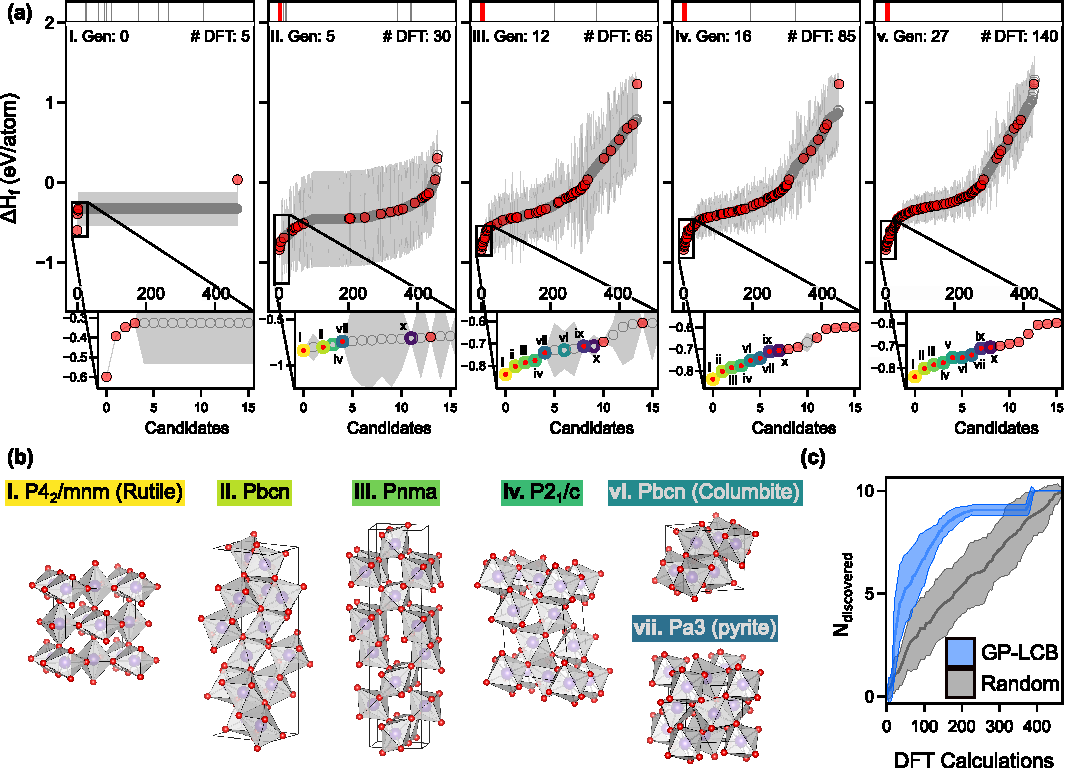
\includegraphics
{02_figures/SI_figures/00_ml_plot_iro2_al__v7__downsampled_1000x1000.pdf}}
\caption{\label{fig:iro2_al}
%
Results for the active learning algorithm applied to the \IrOtwo space.
%
Analogous to Figure \ref{fig:iro3_al}, see Figure \ref{fig:iro3_al} for description of all subplots.
}
\end{figure*}
% __| =====================================================
% =========================================================


% %%%%%%%%%%%%%%%%%%%%%%%%%%%%%%%%%%%%%%%%%%%%%%%%%%%%%%%%%
\subsection{Discovery rate of all runs of AL algorithms} %%
% %%%%%%%%%%%%%%%%%%%%%%%%%%%%%%%%%%%%%%%%%%%%%%%%%%%%%%%%%
% TEMP
% %%%%%%%%%%%%%%%%%%%%%%%%%%%%%%%%%%%%%%%%%%%%%%%%%%%%%%%%%
% | - Discovery rate of all runs of AL algorithms


% %%%%%%%%%%%%%%%%%%%%%%%%%%%%%%%%%%%%%%%%%%%%%%%%%%%%%%%%%
% | - TEMP
%
% __|
% %%%%%%%%%%%%%%%%%%%%%%%%%%%%%%%%%%%%%%%%%%%%%%%%%%%%%%%%%
% | - PARAGRAPH BODY
%
TEMP section
% __|
%%%%%%%%%%%%%%%%%%%%%%%%%%%%%%%%%%%%%%%%%%%%%%%%%%%%%%%%%%%


% __|


% =========================================================
% FIGURE ==================================================
% =========================================================
% | - Figure | Discovery rate of all runs of AL algorithms
\begin{figure*}[!htb]
\centering
\makebox[\textwidth][c]{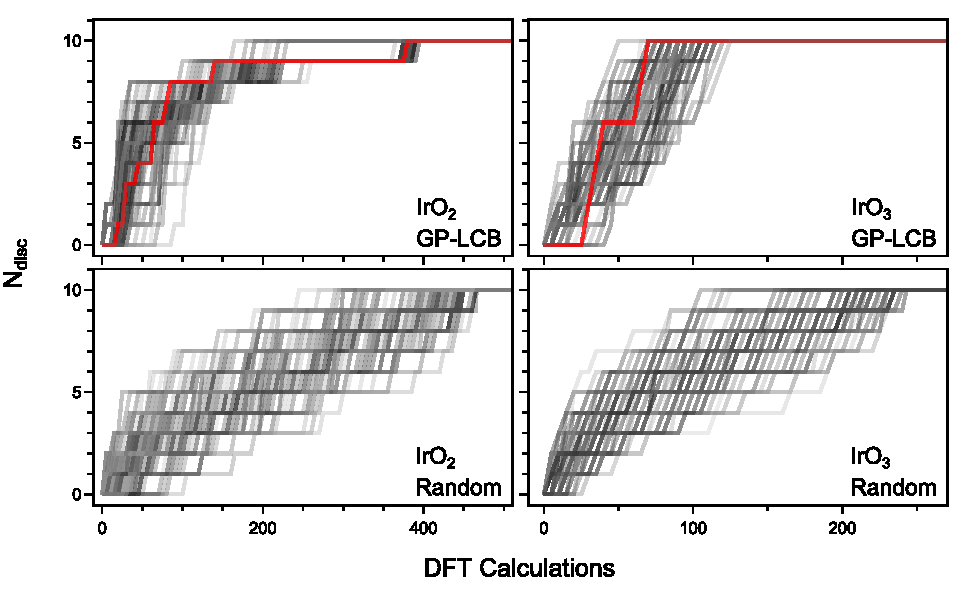
\includegraphics
{02_figures/SI_figures/00_disc_vs_dft__v1.pdf}}
\caption{\label{fig:disc_rate}
%
Quantity of top ten most stable \IrOtwo and \IrOthree polymorphs discovered ($N_{disc}$) as a function of the number of DFT bulk optimizations performed for the GP-LCB acquisition and the baseline random acquisition methods.
%
Red lines indicate the specific runs used for Figures \ref{fig:iro3_al} and Figure \ref{fig:iro2_al}.
}
\end{figure*}
% __| =====================================================
% =========================================================


% %%%%%%%%%%%%%%%%%%%%%%%%%%%%%%%%%%%%%%%%%%%%%%%%%%%%%%%%%
\subsection{Structural coordination motif identification} %
% %%%%%%%%%%%%%%%%%%%%%%%%%%%%%%%%%%%%%%%%%%%%%%%%%%%%%%%%%
%
% %%%%%%%%%%%%%%%%%%%%%%%%%%%%%%%%%%%%%%%%%%%%%%%%%%%%%%%%%
% | - Structural coordination motif identification


% %%%%%%%%%%%%%%%%%%%%%%%%%%%%%%%%%%%%%%%%%%%%%%%%%%%%%%%%%
% | - TEMP
%
% __|
% %%%%%%%%%%%%%%%%%%%%%%%%%%%%%%%%%%%%%%%%%%%%%%%%%%%%%%%%%
% | - PARAGRAPH BODY
TEMP section about doing the structural motiff analysis. Maybe not needed.
% __|
%%%%%%%%%%%%%%%%%%%%%%%%%%%%%%%%%%%%%%%%%%%%%%%%%%%%%%%%%%%


% __|


% %%%%%%%%%%%%%%%%%%%%%%%%%%%%%%%%%%%%%%%%%%%%%%%%%%%%%%%%%
\subsection{Amorphous phase meta-stability analysis} %%%%%%
% %%%%%%%%%%%%%%%%%%%%%%%%%%%%%%%%%%%%%%%%%%%%%%%%%%%%%%%%%
%
% %%%%%%%%%%%%%%%%%%%%%%%%%%%%%%%%%%%%%%%%%%%%%%%%%%%%%%%%%
% | - Amorphous phase meta-stability analysis

% %%%%%%%%%%%%%%%%%%%%%%%%%%%%%%%%%%%%%%%%%%%%%%%%%%%%%%%%%
% | - TEMP
%
% __|
% %%%%%%%%%%%%%%%%%%%%%%%%%%%%%%%%%%%%%%%%%%%%%%%%%%%%%%%%%
% | - PARAGRAPH BODY
The meta-stability analysis based on an ensemble of meta-stable phases developed by TEMP was utlized to set a physically motivated energy cut-off relative to the hull to evaluate the synthesizability of our hypothetical polymorphs.
% __|
%%%%%%%%%%%%%%%%%%%%%%%%%%%%%%%%%%%%%%%%%%%%%%%%%%%%%%%%%%%

% __|

% __|


% #########################################################
\section{Electrochemical OER Computational Methods}  % ####
% #########################################################
%
% #########################################################
% | - Electrochemical OER Computational Methods

% %%%%%%%%%%%%%%%%%%%%%%%%%%%%%%%%%%%%%%%%%%%%%%%%%%%%%%%%%
\subsection{Density Functional Theory Methods}  % %%%%%%%%%
% %%%%%%%%%%%%%%%%%%%%%%%%%%%%%%%%%%%%%%%%%%%%%%%%%%%%%%%%%
%
% %%%%%%%%%%%%%%%%%%%%%%%%%%%%%%%%%%%%%%%%%%%%%%%%%%%%%%%%%
% | - Density Functional Theory Methods
%
All OER calculations were performed using density functional theory (DFT) implemented via the Vienna \latin{ab-initio} simulation package (VASP)
\cite{Kresse1995,Kresse1996_0,Kresse1996_1}
and utilizing the PBE exchange-correlation functional\cite{Perdew1996}.
%
Dipole corrections were imposed on all non-symmetric slabs to counteract spurious dipole interactions between the periodic cells.\cite{Neugebauer1992}
%
% TODO COMBAK, make this section more general, k-points were treated differently
% for different calculations
A 4x4x3 k-point mesh with gamma-point centered Monkshort-packing\cite{Monkhorst1976} was used for all slabs.
%
The plane-wave energy cutoff was \SI{500}{\electronvolt}.
%
% COMBAK Figure out how much spacing was used for all slabs
All slab calculations maintained a vacuum spacing in between TEMP and \SI{15}{\angstrom}
%
All structures were relaxed with utilizing the conjugate gradient algorithm as implemented in VASP (IBRION\num{=2}).
%
The simulation stop criteria used was that all atoms must satisfy a maximum force threshold of \SI{0.02}{\electronvolt\per\angstrom}.
% __|


% %%%%%%%%%%%%%%%%%%%%%%%%%%%%%%%%%%%%%%%%%%%%%%%%%%%%%%%%%
\subsection{Bulk Pourbaix Diagram}  % %%%%%%%%%%%%%%%%%%%%%
% %%%%%%%%%%%%%%%%%%%%%%%%%%%%%%%%%%%%%%%%%%%%%%%%%%%%%%%%%
%
% %%%%%%%%%%%%%%%%%%%%%%%%%%%%%%%%%%%%%%%%%%%%%%%%%%%%%%%%%
% | - Bulk Pourbaix Diagram
%
The electrochemical bulk Pourbaix diagrams were constructed using the TEMP module from pymatgen.
% __|


% =========================================================
% FIGURE ==================================================
% =========================================================
% | - Figure | Bulk Pourbaix Diagram
\begin{figure*}[!htb]
\centering
\makebox[\textwidth][c]{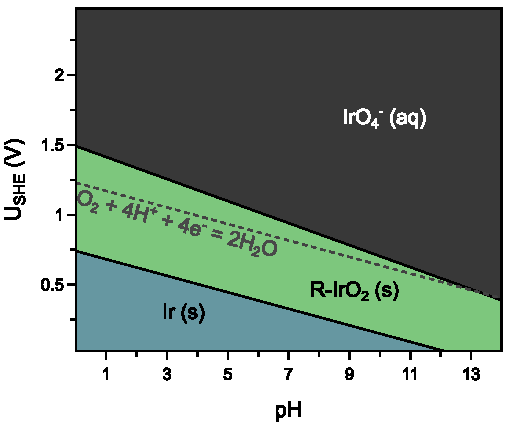
\includegraphics
{02_figures/SI_figures/00_master__bulk-pourbaix__v5.pdf}}
\caption{\label{fig:bulk_pourbaix_wo_alpha}
%
Bulk Pourbaix diagram of the \ce{Ir}-\ce{H2O} system as a function of the applied potential and pH.
%
The diagram was constructed using all of the same species as Figure \ref{fig:bulk_pourbaix} with the exception of the globally stable \IrOthree (\aIrOthree) polymorph.
%
%
% Revised bulk Pourbaix diagram of the \ce{Ir}-\ce{H2O} system as a function of applied potential and pH.
% %
% The diagram was constructed with Ir(s) (blue), \rIrOtwo (green), various \IrOthree polymorphs and a dissolved \ce{IrO^{4-}} ion species (dark grey).
% %
% The stability regions corresponding to the metastable \rIrOthree and \bIrOthree polymorphs, in the absence of any competing \IrOthree phase, are displayed as yellow and pink lines, respectively.
% %
% The thermodynamic onset of OER (water equilibrium at 1.23 \VRHE) is also shown.
}
\end{figure*}
% __| =====================================================
% =========================================================


% %%%%%%%%%%%%%%%%%%%%%%%%%%%%%%%%%%%%%%%%%%%%%%%%%%%%%%%%%
\subsection{OER Thermodynamic Methodology}  % %%%%%%%%%%%%%
% %%%%%%%%%%%%%%%%%%%%%%%%%%%%%%%%%%%%%%%%%%%%%%%%%%%%%%%%%
%
% %%%%%%%%%%%%%%%%%%%%%%%%%%%%%%%%%%%%%%%%%%%%%%%%%%%%%%%%%
% | - OER Thermodynamic Methodology
%
Here we will outline the procedure used to carry out OER simulations on the various slabs of \IrOtwo and \IrOthree.
%
The procedure was as follows:
%
Stable stoichiometric terminations were cut from the bulk.
%
% COMBAK
% TODO Add Vesta reference
Stable termination planes were guesstimated via intuition, and the x-ray diffraction pattern tool from Vesta.
%
Next, electrochemical surface coverage was elucidated via a surface Pourbaix analysis.
%
This elucidates the coverage under operating conditions ($>$\num{1.23} \VRHE) for each slab.
%
% COMBAK
Finally we conducted a thermodynamic/limiting potential analysis of the OER mechanistic pathway (Volcano plot, limiting potentials, etc.).
% __|


% %%%%%%%%%%%%%%%%%%%%%%%%%%%%%%%%%%%%%%%%%%%%%%%%%%%%%%%%%
\subsection{Surface Energy Pourbaix Methodology}  % %%%%%%%
% %%%%%%%%%%%%%%%%%%%%%%%%%%%%%%%%%%%%%%%%%%%%%%%%%%%%%%%%%
%
% %%%%%%%%%%%%%%%%%%%%%%%%%%%%%%%%%%%%%%%%%%%%%%%%%%%%%%%%%
% | - Surface Energy Pourbaix Methodology
%
Surface energy Pourbaix plots were constructed by calculating the surface energy of each slab by under standard conditions (\si{\volt}\num{=0} and pH\num{=0}) and then utilizing the computational hydrogen electrode (CHE) to compute the potential dependence of the surfaces.
%
Surface energy calculations were performed for various facets for slabs of increasing thickness.
%
% TODO Insert reference for surface E calcs
The bulk energy was then extracted by fitting the total energy of the slabs against the number of layers as explained in TEMP.
%
This was  done to avoid common issues of surface energy divergence associated with using a separate bulk energy calculation.
%
The sensitivity of a given slab to an applied bias is dependent on the composition of the surface,
in particular, the effect of coverage of electrolyte species which can deposit oxygen, hydrogen, and hydroxide species on the surface layers.
%
These additional \ce{O} and \ce{H} atoms are not referenced to the atoms in the slab, but are instead referenced to the computational hydrogen electrode and water-splitting reaction.
%
% TODO Type out equations for surface energy calculation
The equation for is as follows:
% __|


% %%%%%%%%%%%%%%%%%%%%%%%%%%%%%%%%%%%%%%%%%%%%%%%%%%%%%%%%%
\subsection{OER Scaling Relations}  % %%%%%%%%%%%%%%%%%%%%%
% %%%%%%%%%%%%%%%%%%%%%%%%%%%%%%%%%%%%%%%%%%%%%%%%%%%%%%%%%
%
% %%%%%%%%%%%%%%%%%%%%%%%%%%%%%%%%%%%%%%%%%%%%%%%%%%%%%%%%%
% %%%%%%%%%%%%%%%%%%%%%%%%%%%%%%%%%%%%%%%%%%%%%%%%%%%%%%%%%
% | - OER Scaling Relations


% %%%%%%%%%%%%%%%%%%%%%%%%%%%%%%%%%%%%%%%%%%%%%%%%%%%%%%%%%
% | - TEMP
%
% __|
% %%%%%%%%%%%%%%%%%%%%%%%%%%%%%%%%%%%%%%%%%%%%%%%%%%%%%%%%%
% | - PARAGRAPH BODY
%
Figure~\ref{fig:scaling_relations} shows the scaling relations between the adsorption free energies of the OER intermediate species for the studied \IrOx slabs.
%
It can be seen clearly that the data points corresponding to the three \IrOthree polymorphs are roughly \SI{1}{\electronvolt} weaker binding than the \rIrOtwo points.
%
This generally weaker binding of the \IrOthree stoichiometry is responsible for the observed improvement in theoretical activity.
%
The \DGOOH vs.\DGOH relationship is very close to the traditional ``universal scaling relations'', demonstrating that our materials do not break the infamous \DGOOH vs. \DGOH scaling.

% __|
%%%%%%%%%%%%%%%%%%%%%%%%%%%%%%%%%%%%%%%%%%%%%%%%%%%%%%%%%%%


% __|


% =========================================================
% FIGURE ==================================================
% =========================================================
% | - Figure | OER Scaling Relations
\begin{figure*}[!htb]
\centering
\makebox[\textwidth][c]{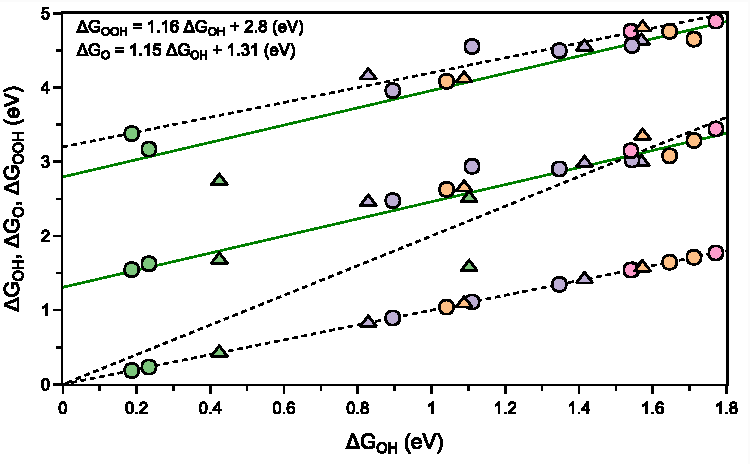
\includegraphics
{02_figures/SI_figures/00_master__oer_scaling__main_v3.pdf}}
\caption{\label{fig:scaling_relations}
%
Relationship between the adsorption free energies of the three key OER intermediates (*OH, *O, *OOH), with \DGOH chosen as the dependent variable.
%
Best fit lines are provided for \DGOOH vs. \DGOH and \DGO vs. \DGOH.
%
Additionally, ``universal scaling relations'' for \DGOOH vs. \DGOH and \DGO vs. \DGOH are shown (black dotted lines) to emphasize our deviation from the traditionally reported scaling fits.
%
The \DGOH line is  shown as guide to eye.
% TODO Do I have to redefine the color convention every caption?
}
\end{figure*}
% __| =====================================================
% =========================================================


% %%%%%%%%%%%%%%%%%%%%%%%%%%%%%%%%%%%%%%%%%%%%%%%%%%%%%%%%%
\subsection{Bulk Systems}  % %%%%%%%%%%%%%%%%%%%%%%%%%%%%%%
% %%%%%%%%%%%%%%%%%%%%%%%%%%%%%%%%%%%%%%%%%%%%%%%%%%%%%%%%%
%
% %%%%%%%%%%%%%%%%%%%%%%%%%%%%%%%%%%%%%%%%%%%%%%%%%%%%%%%%%
% %%%%%%%%%%%%%%%%%%%%%%%%%%%%%%%%%%%%%%%%%%%%%%%%%%%%%%%%%
% | - Bulk Systems


% %%%%%%%%%%%%%%%%%%%%%%%%%%%%%%%%%%%%%%%%%%%%%%%%%%%%%%%%%
% | - TEMP
%
% __|
% %%%%%%%%%%%%%%%%%%%%%%%%%%%%%%%%%%%%%%%%%%%%%%%%%%%%%%%%%
% | - PARAGRAPH BODY
% Formation energies of 4 polymorphs
% __|
%%%%%%%%%%%%%%%%%%%%%%%%%%%%%%%%%%%%%%%%%%%%%%%%%%%%%%%%%%%


% __|


% %%%%%%%%%%%%%%%%%%%%%%%%%%%%%%%%%%%%%%%%%%%%%%%%%%%%%%%%%
\subsection{Table of OER energetics}  % %%%%%%%%%%%%%%%%%%%
% %%%%%%%%%%%%%%%%%%%%%%%%%%%%%%%%%%%%%%%%%%%%%%%%%%%%%%%%%
%
% %%%%%%%%%%%%%%%%%%%%%%%%%%%%%%%%%%%%%%%%%%%%%%%%%%%%%%%%%
% %%%%%%%%%%%%%%%%%%%%%%%%%%%%%%%%%%%%%%%%%%%%%%%%%%%%%%%%%
% | - Table of OER energetics


% %%%%%%%%%%%%%%%%%%%%%%%%%%%%%%%%%%%%%%%%%%%%%%%%%%%%%%%%%
% | - TEMP
%
% __|
% %%%%%%%%%%%%%%%%%%%%%%%%%%%%%%%%%%%%%%%%%%%%%%%%%%%%%%%%%
% | - PARAGRAPH BODY
%
Table \ref{table:oer_data} contains the adsorbate binding energetics for the intermediates of the OER
oxygen evolution reaction (*O, *OOH, *OH).
% __|
%%%%%%%%%%%%%%%%%%%%%%%%%%%%%%%%%%%%%%%%%%%%%%%%%%%%%%%%%%%


% __|


% =========================================================
% TABLE ===================================================
% =========================================================
% | - Table | OER energetics
\newpage  % request a new page.
\begin{landscape}
\renewcommand{\arraystretch}{1.5} % <--------------
\begin{table}
\resizebox{\linewidth}{!}{%
\centering
\caption{\label{table:oer_data}
%
OER adsorbation energies for slabs of \IrOtwo and \IrOthree polymorphs studied here.
%
Included quantities are electronic adsorption energies
($\Delta E_{*O_{x}H_{y}}$),
adsorption free energies
($\Delta G_{*O_{x}H_{y}}$),
as well as the \DGOmOH OER descriptor.
%
Coverage indicates the electrochemical coverage of either *O or *OH species.
%
The limiting potential and corresponding overpotential ($\eta$) as well as the rate determining step (RDS) for the OER mechanism are shown.
}
\begin{tabular}{lllcccccccccc}
\toprule
                Bulk Sys. &    Facet &    Coverage & $\Delta E_{*OH}$ & $\Delta E_{*O}$ & $\Delta E_{*OOH}$ & $\Delta G_{*OH}$ & $\Delta G_{*O}$ & $\Delta G_{*OOH}$ & $\Delta G_{*O}-\Delta G_{*OH}$ & Lim. Pot. & $\eta$ &                                                                    RDS \\
                        - &        - &           - &             (eV) &            (eV) &              (eV) &             (eV) &            (eV) &              (eV) &                           (eV) &       (V) &    (V) &                                                                      - \\
\midrule
      $R{\text -}IrO_{2}$ &    (100) &         *OH &            0.130 &           1.634 &             2.362 &            0.424 &           1.678 &             2.738 &                          1.254 &     2.182 &  0.952 &              $*OOH \rightarrow * \phantom{T} \phantom{T} \phantom{T} $ \\
      $R{\text -}IrO_{2}$ &    (100) &          *O &           -0.061 &           1.582 &             2.793 &            0.234 &           1.626 &             3.170 &                          1.392 &     1.750 &  0.520 &              $*OOH \rightarrow * \phantom{T} \phantom{T} \phantom{T} $ \\
      $R{\text -}IrO_{2}$ &    (110) &         *OH &            0.807 &           1.535 &             2.133 &            1.102 &           1.579 &             2.509 &                          0.477 &     2.411 &  1.181 &              $*OOH \rightarrow * \phantom{T} \phantom{T} \phantom{T} $ \\
      $R{\text -}IrO_{2}$ &    (110) &          *O &           -0.108 &           1.503 &             3.004 &            0.187 &           1.547 &             3.380 &                          1.360 &     1.833 &  0.603 &                         $*O \phantom{T} \phantom{T}  \rightarrow *OOH$ \\
 $\alpha{\text -}IrO_{3}$ &    (100) &         *OH &            1.275 &           2.950 &             4.254 &            1.569 &           2.994 &             4.630 &                          1.424 &     1.636 &  0.406 &                         $*O \phantom{T} \phantom{T}  \rightarrow *OOH$ \\
 $\alpha{\text -}IrO_{3}$ &    (100) &          *O &            1.249 &           2.980 &             4.191 &            1.544 &           3.024 &             4.567 &                          1.480 &     1.544 &  0.314 &  $* \phantom{T} \phantom{T} \phantom{T}  \rightarrow *OH \phantom{T} $ \\
 $\alpha{\text -}IrO_{3}$ &    (110) &         *OH &            0.534 &           2.414 &             3.786 &            0.828 &           2.458 &             4.163 &                          1.629 &     1.705 &  0.475 &                         $*O \phantom{T} \phantom{T}  \rightarrow *OOH$ \\
 $\alpha{\text -}IrO_{3}$ &    (110) &          *O &            0.600 &           2.432 &             3.582 &            0.895 &           2.476 &             3.959 &                          1.581 &     1.581 &  0.351 &              $*OH \phantom{T} \rightarrow *O \phantom{T} \phantom{T} $ \\
 $\alpha{\text -}IrO_{3}$ &    (111) &          *O &            0.815 &           2.894 &             4.177 &            1.110 &           2.938 &             4.554 &                          1.828 &     1.828 &  0.598 &              $*OH \phantom{T} \rightarrow *O \phantom{T} \phantom{T} $ \\
 $\alpha{\text -}IrO_{3}$ &    (211) &         *OH &            1.120 &           2.937 &             4.173 &            1.415 &           2.981 &             4.549 &                          1.566 &     1.568 &  0.338 &                         $*O \phantom{T} \phantom{T}  \rightarrow *OOH$ \\
 $\alpha{\text -}IrO_{3}$ &    (211) &          *O &            1.052 &           2.860 &             4.122 &            1.347 &           2.904 &             4.499 &                          1.558 &     1.594 &  0.364 &                         $*O \phantom{T} \phantom{T}  \rightarrow *OOH$ \\
  $\beta{\text -}IrO_{3}$ &  (010)-A &          *O &            1.246 &           3.105 &             4.383 &            1.541 &           3.149 &             4.759 &                          1.609 &     1.610 &  0.380 &                         $*O \phantom{T} \phantom{T}  \rightarrow *OOH$ \\
  $\beta{\text -}IrO_{3}$ &  (010)-B &          *O &            1.477 &           3.399 &             4.519 &            1.771 &           3.443 &             4.896 &                          1.672 &     1.771 &  0.541 &  $* \phantom{T} \phantom{T} \phantom{T}  \rightarrow *OH \phantom{T} $ \\
      $R{\text -}IrO_{3}$ &    (100) &         *OH &            1.278 &           3.304 &             4.431 &            1.572 &           3.348 &             4.807 &                          1.776 &     1.776 &  0.546 &              $*OH \phantom{T} \rightarrow *O \phantom{T} \phantom{T} $ \\
      $R{\text -}IrO_{3}$ &    (100) &          *O &            1.351 &           3.036 &             4.381 &            1.646 &           3.080 &             4.758 &                          1.435 &     1.677 &  0.447 &                         $*O \phantom{T} \phantom{T}  \rightarrow *OOH$ \\
      $R{\text -}IrO_{3}$ &    (100) &  *O-partial &            1.417 &           3.243 &             4.275 &            1.712 &           3.287 &             4.652 &                          1.575 &     1.712 &  0.482 &  $* \phantom{T} \phantom{T} \phantom{T}  \rightarrow *OH \phantom{T} $ \\
      $R{\text -}IrO_{3}$ &    (110) &         *OH &            0.794 &           2.607 &             3.744 &            1.088 &           2.651 &             4.121 &                          1.563 &     1.563 &  0.333 &              $*OH \phantom{T} \rightarrow *O \phantom{T} \phantom{T} $ \\
      $R{\text -}IrO_{3}$ &    (110) &          *O &            0.746 &           2.583 &             3.708 &            1.041 &           2.627 &             4.084 &                          1.586 &     1.586 &  0.356 &              $*OH \phantom{T} \rightarrow *O \phantom{T} \phantom{T} $ \\
\bottomrule
\end{tabular}

}
\end{table}

\end{landscape}
% __| =====================================================
% =========================================================

% __|

\end{suppinfo}
% __|

% | - Bibliography ************************************************************
\bibliography{%
01_references/global_opt_refs.bib,%
01_references/irox_refs.bib,%
01_references/misc_refs.bib,%
01_references/ml_refs.bib,%
01_references/oer_refs.bib,%
01_references/software_refs.bib,%
}
% __|

\end{document}
